
%%%%%%%%%%%%%%%%%%%%%%%%%%%%%%%%%%%%%%%%%%%%%%%%%%
%%%%%%%%%%%%%%%%%%%%% preamble %%%%%%%%%%%%%%%%%%%
%%%%%%%%%%%%%%%%%%%%%%%%%%%%%%%%%%%%%%%%%%%%%%%%%%
\documentclass[11pt,twoside]{book}
\usepackage[mono=false]{libertine} % new linux font, ignore mono

\usepackage{luatex85}

%\renewcommand{\baselinestretch}{1.05}
\usepackage{amsmath,amsthm,amssymb,mathrsfs,amsfonts,dsfont}
\usepackage{epsfig,graphicx}
\usepackage{tabularx}
\usepackage{blkarray}
\usepackage{slashed}
\usepackage{color}
\usepackage{listings}
\lstset{
    language=bash,
    basicstyle=\ttfamily,
    breaklines=true,
    showstringspaces=false,
    commentstyle=\color{green!40!black},
    keywordstyle=\color{blue},
    stringstyle=\color{orange}
}
\usepackage{caption}
% \usepackage{fullpage}
\usepackage{lipsum} % provides dummy text for testing
\usepackage[toc,title,titletoc,header]{appendix}
\usepackage{minitoc}
\usepackage{color}
\usepackage{multicol} % two-col ToC
\usepackage{bm}
\usepackage{imakeidx} % before hyperref
\usepackage{hyperref}
\usepackage{url}
\captionsetup[figure]{name=Imagen}
% link colors settings
\hypersetup{
    colorlinks=true,
    citecolor=magenta,
    linkcolor=black,
    filecolor=green,      
    urlcolor=cyan,
    % hypertexnames=false,
}
\usepackage[capitalise]{cleveref}
\usepackage{subcaption}
\usepackage{enumitem}
\usepackage{mathtools}
\usepackage{physics}
\usepackage[linesnumbered,ruled,vlined,algosection]{algorithm2e}
\SetCommentSty{textsf}
\usepackage{epigraph}
\epigraphwidth=1.0\linewidth
\epigraphrule=0pt

% adjust margin
\usepackage[margin=2.3cm]{geometry}
\headheight13.6pt

%%%%%%%%%%%%%%%% thmtools %%%%%%%%%%%%%%%%%%%%%
\usepackage{thmtools}
\declaretheorem[numberwithin=chapter]{theorem}
\declaretheorem[numberwithin=chapter]{axiom}
\declaretheorem[numberwithin=chapter]{lemma}
\declaretheorem[numberwithin=chapter]{proposition}
\declaretheorem[numberwithin=chapter]{claim}
\declaretheorem[numberwithin=chapter]{conjecture}
\declaretheorem[sibling=theorem]{corollary}
\declaretheorem[numberwithin=chapter, style=definition]{definition}
\declaretheorem[numberwithin=chapter, style=definition]{problem}
\declaretheorem[numberwithin=chapter, style=definition]{example}
\declaretheorem[numberwithin=chapter, style=definition]{exercise}
\declaretheorem[numberwithin=chapter, style=definition]{observation}
\declaretheorem[numberwithin=chapter, style=definition]{fact}
\declaretheorem[numberwithin=chapter, style=definition]{construction}
\declaretheorem[numberwithin=chapter, style=definition]{remark}
\declaretheorem[numberwithin=chapter, style=remark]{question}
%%%%%%%%%%%%%%%% thmtools %%%%%%%%%%%%%%%%%%%%%
\usepackage{changepage}
\newenvironment{solution}
    {\renewcommand\qedsymbol{$\square$}\color{blue}\begin{adjustwidth}{0em}{2em}\begin{proof}[\textit Solution.~]}
    {\end{proof}\end{adjustwidth}}

%%%%%%%%%%%%%%%% index %%%%%%%%%%%%%%%%%%%%%
\begin{filecontents}{index.ist}
% https://tex.stackexchange.com/questions/65247/index-with-an-initial-letter-of-the-group
headings_flag 1
heading_prefix "{\\centering\\large \\textbf{"
heading_suffix "}}\\nopagebreak\n"
delim_0 "\\nobreak\\dotfill"
\end{filecontents}
\newcommand{\myindex}[1]{\index{#1} \emph{#1}}
\makeindex[columns=3, intoc, title=Alphabetical Index, options= -s index.ist]
%%%%%%%%%%%%%%%% index %%%%%%%%%%%%%%%%%%%%%

%%%%%%%%%%%%%%%% ToC %%%%%%%%%%%%%%%%%%%%%
% Link Chapter title to ToC: https://tex.stackexchange.com/questions/32495/linking-the-section-text-to-the-toc
\usepackage[explicit]{titlesec}
\titleformat{\chapter}[display]
  {\normalfont\huge\bfseries}{\chaptertitlename\ {\thechapter}}{20pt}{\hyperlink{chap-\thechapter}{\Huge#1}
\addtocontents{toc}{\protect\hypertarget{chap-\thechapter}{}}}
\titleformat{name=\chapter,numberless}
  {\normalfont\huge\bfseries}{}{-20pt}{\Huge#1}

%%%%%%%%%%%%%%%%%%% fancyhdr %%%%%%%%%%%%%%%%%
\usepackage{fancyhdr}
\pagestyle{fancy} % enable fancy page style
\renewcommand{\headrulewidth}{0.0pt} % comment if you want the rule
\fancyhf{} % clear header and footer
\fancyhead[lo,le]{\leftmark}
\fancyhead[re,ro]{\rightmark}
\fancyfoot[CE,CO]{\hyperref[toc-contents]{\thepage}}

% https://tex.stackexchange.com/questions/550520/making-each-page-number-link-back-to-beginning-of-chapter-or-section
\makeatletter
\def\chaptermark#1{\markboth{\protect\hyper@linkstart{link}{\@currentHref}{Chapter \thechapter ~ #1}\protect\hyper@linkend}{}}
\def\sectionmark#1{\markright{\protect\hyper@linkstart{link}{\@currentHref}{\thesection ~ #1}\protect\hyper@linkend}}
\makeatother
%%%%%%%%%%%%%%%%%%% fancyhdr %%%%%%%%%%%%%%%%%


%%%%%%%%%%%%%%%%%%% biblatex %%%%%%%%%%%%%%%%%
\usepackage[doi=false,url=false,isbn=false,style=alphabetic,backend=biber,backref=true]{biblatex}
\addbibresource{bib.bib}

\newbibmacro{string+doiurlisbn}[1]{%
  \iffieldundef{doi}{%
    \iffieldundef{url}{%
      \iffieldundef{isbn}{%
        \iffieldundef{issn}{%
          #1%
        }{%
          \href{http://books.google.com/books?vid=ISSN\thefield{issn}}{#1}%
        }%
      }{%
        \href{http://books.google.com/books?vid=ISBN\thefield{isbn}}{#1}%
      }%
    }{%
      \href{\thefield{url}}{#1}%
    }%
  }{%
    \href{http://dx.doi.org/\thefield{doi}}{#1}%
  }%
}

% https://tex.stackexchange.com/questions/94089/remove-quotes-from-inbook-reference-title-with-biblatex
\DeclareFieldFormat[article,incollection,inproceedings,book,misc]{title}{\usebibmacro{string+doiurlisbn}{\mkbibemph{#1}}}
% https://tex.stackexchange.com/questions/454672/biblatex-journal-name-non-italic
\DeclareFieldFormat{journaltitle}{#1\isdot}
\DeclareFieldFormat{booktitle}{#1\isdot}
% https://tex.stackexchange.com/questions/10682/suppress-in-biblatex
\renewbibmacro{in:}{}
% add video field: https://tex.stackexchange.com/questions/111846/biblatex-2-custom-fields-only-one-is-working
\DeclareSourcemap{
    \maps[datatype=bibtex]{
      \map{
        \step[fieldsource=video]
        \step[fieldset=usera,origfieldval]
    }
  }
}
\DeclareFieldFormat{usera}{\href{#1}{\textsc{Online video}}}
\AtEveryBibitem{
    \csappto{blx@bbx@\thefield{entrytype}}{% put at end of entry
        \iffieldundef{usera}{}{\space \printfield{usera}}
    }
}
%%%%%%%%%%%%%%%%%%% biblatex %%%%%%%%%%%%%%%%%

%%%%%%%%%%%%%%%%%%%%% glossaries %%%%%%%%%%%%%%%%%
% !TEX root = ./notes_template.tex
% \usepackage[style=super]{glossaries}
% https://www.overleaf.com/learn/latex/Glossaries
\usepackage[style=super,toc,acronym]{glossaries}
\setlength{\glsdescwidth}{1\linewidth}
\makeglossaries

\renewcommand\glossaryname{List of Abbreviations and Symbols}

\newglossaryentry{Q2}{name={$Q_2(f)$},
%sort=Q2,
description={Two-side (bounded) error quantum query complexity}}

\newglossaryentry{real_number}{name={$\mathbb{R}$},description={Real number}}

% \newglossaryentry{gcd}{name={gcd},description={greatest common divisor}}

\newacronym{gcd}{GCD}{Greatest Common Divisor}


\newglossaryentry{svm}{name={SVM},description={Support Vector Machine}}

\newglossaryentry{gd}{name={GD},description={Gradient Descent}}

\newglossaryentry{qft}{name={QFT},description={Quantum Field Theory}}

\newglossaryentry{qm}{name={QM},description={Quantum Mechanics}}

\newglossaryentry{v}{name={$\vec{v}$},description={a vector}}

% physics
\newglossaryentry{hamiltonian}{name={$\hat{H}$},description={Hamiltonian}}

\newglossaryentry{lagrangian}{name={$L$},description={Lagrangian}}
%%%%%%%%%%%%%%%%%%%%% glossaries %%%%%%%%%%%%%%%%%

%%%%%%%%%%%%%%%%%%%%% glossaries-extra %%%%%%%%%%%%%%%%%
% \usepackage[record,abbreviations,symbols,stylemods={list,tree,mcols}]{glossaries-extra}
%%%%%%%%%%%%%%%%%%%%% glossaries-extra %%%%%%%%%%%%%%%%%


% !TEX root = ./notes_template.tex
%%%%%%%%%%%%%%%%%%%%%%%%%%%%%%%%%%%%%%%%%%%%%%%%%%
%%%%%%%%%%%%%%%%%%%%% preamble %%%%%%%%%%%%%%%%%%%
%%%%%%%%%%%%%%%%%%%%%%%%%%%%%%%%%%%%%%%%%%%%%%%%%%
\usepackage[mono=false]{libertine} % new linux font, ignore mono

\usepackage{luatex85}

%\renewcommand{\baselinestretch}{1.05}
\usepackage{amsmath,amsthm,amssymb,mathrsfs,amsfonts,dsfont}
\usepackage{epsfig,graphicx}
\usepackage{tabularx}
\usepackage{blkarray}
\usepackage{slashed}
\usepackage{color}
\usepackage{listings}
\usepackage{caption}
% \usepackage{fullpage}
\usepackage{lipsum} % provides dummy text for testing
\usepackage[toc,title,titletoc,header]{appendix}
\usepackage{minitoc}
\usepackage{color}
\usepackage{multicol} % two-col ToC
\usepackage{bm}
\usepackage{imakeidx} % before hyperref
\usepackage{hyperref}
% link colors settings
\hypersetup{
    colorlinks=true,
    citecolor=magenta,
    linkcolor=black,
    filecolor=green,      
    urlcolor=cyan,
    % hypertexnames=false,
}
\usepackage[capitalise]{cleveref}
\usepackage{subcaption}
\usepackage{enumitem}
\usepackage{mathtools}
\usepackage{physics}
\usepackage[linesnumbered,ruled,vlined,algosection]{algorithm2e}
\SetCommentSty{textsf}
\usepackage{epigraph}
\epigraphwidth=1.0\linewidth
\epigraphrule=0pt

% adjust margin
\usepackage[margin=2.3cm]{geometry}
\headheight13.6pt

%%%%%%%%%%%%%%%% thmtools %%%%%%%%%%%%%%%%%%%%%

%%%%%%%%%%%%%%%% thmtools %%%%%%%%%%%%%%%%%%%%%
\usepackage{changepage}

%%%%%%%%%%%%%%%% index %%%%%%%%%%%%%%%%%%%%%
% https://tex.stackexchange.com/questions/65247/index-with-an-initial-letter-of-the-group
%\makeindex[columns=3, intoc, title=Alphabetical Index, %options= -s index.ist]
%%%%%%%%%%%%%%%% index %%%%%%%%%%%%%%%%%%%%%
%%%%%%%%%%%%%%%% ToC %%%%%%%%%%%%%%%%%%%%%
% Link Chapter title to ToC: https://tex.stackexchange.com/questions/32495/linking-the-section-text-to-the-toc
%\usepackage[explicit]{titlesec}
%\titleformat{\chapter}[display]
 % {\normalfont\huge\bfseries}{\chaptertitlename\ {\thechapter}}{20pt}{\hyperlink{chap-\thechapter}{\Huge#1}
%\addtocontents{toc}{\protect\hypertarget{chap-\thechapter}{}}}
%\titleformat{name=\chapter,numberless}
 % {\normalfont\huge\bfseries}{}{-20pt}{\Huge#1}
%%%%%%%%%%%%%%%%%%% fancyhdr %%%%%%%%%%%%%%%%%
\pagestyle{fancy} % enable fancy page style
\renewcommand{\headrulewidth}{0.0pt} % comment if you want the rule
\fancyhf{} % clear header and footer
\fancyhead[lo,le]{\leftmark}
\fancyhead[re,ro]{\rightmark}
\fancyfoot[CE,CO]{\hyperref[toc-contents]{\thepage}}

% https://tex.stackexchange.com/questions/550520/making-each-page-number-link-back-to-beginning-of-chapter-or-section
\makeatletter
\def\chaptermark#1{\markboth{\protect\hyper@linkstart{link}{\@currentHref}{Chapter \thechapter ~ #1}\protect\hyper@linkend}{}}
\def\sectionmark#1{\markright{\protect\hyper@linkstart{link}{\@currentHref}{\thesection ~ #1}\protect\hyper@linkend}}
\makeatother
%%%%%%%%%%%%%%%%%%% fancyhdr %%%%%%%%%%%%%%%%%


%%%%%%%%%%%%%%%%%%% biblatex %%%%%%%%%%%%%%%%%
\usepackage[doi=false,url=false,isbn=false,style=alphabetic,backend=biber,backref=true]{biblatex}
\addbibresource{bib.bib}

\newbibmacro{string+doiurlisbn}[1]{%
  \iffieldundef{doi}{%
    \iffieldundef{url}{%
      \iffieldundef{isbn}{%
        \iffieldundef{issn}{%
          #1%
        }{%
          \href{http://books.google.com/books?vid=ISSN\thefield{issn}}{#1}%
        }%
      }{%
        \href{http://books.google.com/books?vid=ISBN\thefield{isbn}}{#1}%
      }%
    }{%
      \href{\thefield{url}}{#1}%
    }%
  }{%
    \href{http://dx.doi.org/\thefield{doi}}{#1}%
  }%
}

% https://tex.stackexchange.com/questions/94089/remove-quotes-from-inbook-reference-title-with-biblatex
\DeclareFieldFormat[article,incollection,inproceedings,book,misc]{title}{\usebibmacro{string+doiurlisbn}{\mkbibemph{#1}}}
% https://tex.stackexchange.com/questions/454672/biblatex-journal-name-non-italic
\DeclareFieldFormat{journaltitle}{#1\isdot}
\DeclareFieldFormat{booktitle}{#1\isdot}
% https://tex.stackexchange.com/questions/10682/suppress-in-biblatex
\renewbibmacro{in:}{}
% add video field: https://tex.stackexchange.com/questions/111846/biblatex-2-custom-fields-only-one-is-working
\DeclareSourcemap{
    \maps[datatype=bibtex]{
      \map{
        \step[fieldsource=video]
        \step[fieldset=usera,origfieldval]
    }
  }
}
\DeclareFieldFormat{usera}{\href{#1}{\textsc{Online video}}}
\AtEveryBibitem{
    \csappto{blx@bbx@\thefield{entrytype}}{% put at end of entry
        \iffieldundef{usera}{}{\space \printfield{usera}}
    }
}
%%%%%%%%%%%%%%%%%%% biblatex %%%%%%%%%%%%%%%%%

%%%%%%%%%%%%%%%%%%%%% glossaries %%%%%%%%%%%%%%%%%
%% !TEX root = ./notes_template.tex
% \usepackage[style=super]{glossaries}
% https://www.overleaf.com/learn/latex/Glossaries
\usepackage[style=super,toc,acronym]{glossaries}
\setlength{\glsdescwidth}{1\linewidth}
\makeglossaries

\renewcommand\glossaryname{List of Abbreviations and Symbols}

\newglossaryentry{Q2}{name={$Q_2(f)$},
%sort=Q2,
description={Two-side (bounded) error quantum query complexity}}

\newglossaryentry{real_number}{name={$\mathbb{R}$},description={Real number}}

% \newglossaryentry{gcd}{name={gcd},description={greatest common divisor}}

\newacronym{gcd}{GCD}{Greatest Common Divisor}


\newglossaryentry{svm}{name={SVM},description={Support Vector Machine}}

\newglossaryentry{gd}{name={GD},description={Gradient Descent}}

\newglossaryentry{qft}{name={QFT},description={Quantum Field Theory}}

\newglossaryentry{qm}{name={QM},description={Quantum Mechanics}}

\newglossaryentry{v}{name={$\vec{v}$},description={a vector}}

% physics
\newglossaryentry{hamiltonian}{name={$\hat{H}$},description={Hamiltonian}}

\newglossaryentry{lagrangian}{name={$L$},description={Lagrangian}}
%%%%%%%%%%%%%%%%%%%%% glossaries %%%%%%%%%%%%%%%%%

%%%%%%%%%%%%%%%%%%%%% glossaries-extra %%%%%%%%%%%%%%%%%
% \usepackage[record,abbreviations,symbols,stylemods={list,tree,mcols}]{glossaries-extra}
%%%%%%%%%%%%%%%%%%%%% glossaries-extra %%%%%%%%%%%%%%%%%


% !TEX root = ./notes_template.tex

%%%%%%%%%%%%%%%%%%%%%%%%%%%%%%%%%%%%
%%%%%%%%%%%%%%%%%%%%%%%%%%%%%%%%%%%%
% math
\let\iff\relax
\newcommand{\iff}{\text{ iff }}
\newcommand{\OPT}{\textup{OPT}}

% physics
\newcommand{\acreation}{a^\dagger}



%%%%%%%%%%%%%%%%%%%%%%%%%%%%%%%%%%%%%%%%%%%%%%%%%%
%%%%%%%%%%%%%%%% begin of document %%%%%%%%%%%%%%%
%%%%%%%%%%%%%%%%%%%%%%%%%%%%%%%%%%%%%%%%%%%%%%%%%%


\usepackage{graphicx}
\usepackage{multicol}
\usepackage{xcolor}
\usepackage{titletoc}
\usepackage{hyperref}
\usepackage[utf8]{inputenc}
\usepackage[spanish]{babel}
\addto\captionsspanish{\renewcommand{\figurename}{Figura}}


\begin{document}

% Portada
\begin{center}
  \LARGE UNIVERSIDAD DE LAS FUERZAS ARMADAS ESPE\\[0.5cm]
  \Large DEPARTAMENTO CIENCIAS DE LA COMPUTACIÓN \\[0.5cm]
  \large SISTEMAS OPERATIVOS\\[0.5cm]
  \begin{figure}[htb] \centering 
\includegraphics[scale=.6]{Logo_ESPE} \end{figure}
   \vspace{0.5cm}
  \large{\bf CUADERNO VIRTUAL }\\ \vspace{.25cm} 
\end{center}

\begin{flushleft}
  \Large{\bf NRC: } 14912 \textbf{}\\
  \vspace{0.5cm}
  \Large{\bf Carrera:} Ingeniería de Software\\
  \vspace{0.5cm}
  \Large{\bf Nombre: } Gustavo Aguas\\
  \vspace{0.5cm}
  \Large{\bf Docente: } Ing. Fuertes Diaz Walter Marcelo Dr.\\
  \vspace{0.5cm}
  %\Large{\bf Grupo: }
  \vspace{0.5cm}
\end{flushleft}

\begin{center} \Large \textsc{Sangolqui - Ecuador} \\
\vspace{0.5cm}
  \Large \textsc{2024 } \end{center}

\let\cleardoublepage\clearpage

% Tabla de Contenido de una sola columna
\begin{center}
  %\Large\textbf{Table of Contents}
  %\thispagestyle{empty} % Eliminar encabezado y pie de página
  %\dominitoc % Inicialización
  \tableofcontents
  \label{toc-contents}
\end{center}
\clearpage % Forzar un salto de página

% Establecer numeración de capítulos a partir de 1
\setcounter{chapter}{0}
\renewcommand{\thechapter}{\arabic{chapter}}

% Desactivar minitoc antes de Secciones
\adjustmtc
\setcounter{mtc}{0}
\clearpage
% Secciones y contenido
\chapter{Materia}
En este cuaderno virtual desempeña un papel fundamental al proporcionar una guía completa de los temas que seran abordados a lo largo del semestre. Su función es trascender más alla de un registro de la materia, convirtiendose en una herramienta esencial para la preparación y estudio. Ademas de presentar teoría, sera un recurso indispensable para la realización de prácticas y actividades, fomentando la aplicación practica de los cononomientos adquiridos en clase. Con el proposito de facilitar el proceso de aprendizaje, brindando una estructura organizada que potencia la comprensión.
\section{Fundamentos de Sistema Operativo}

Es un conjunto de programas de software que permiten administrar los recursos computacionales.
\begin{itemize}
  \item CPU
  \item RAM
  \item Almacenamiento
  \item I/D Devices
  \end{itemize}
El sistema operativo de una computadora es un software muy importante que controla los recursos de hardware y software al mismo tiempo que proporciona los servicios necesarios a los programas de computadora. Actúa como intermediario entre los componentes de hardware y software de un sistema informático, permitiendo la comunicación y coordinación entre ellos. El propósito principal de un sistema operativo es crear un entorno de computación conveniente y eficiente para los usuarios, al mismo tiempo que se garantiza el uso más eficiente de los recursos disponibles.  



\begin{figure}[htb]
  \centering
  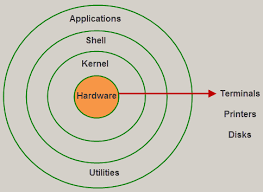
\includegraphics[width=0.8\linewidth]{A.L.png}
  \caption{Arquitectura de Linux}
  \label{fig:etiqueta}
\end{figure}

\newpage
\section{Ejemplos}

\begin{itemize}
  \item Microsoft Windows 11 --- Bill Gates
  \item MacOs --- Steve Jobs Dennis Ritchie
  \item Android --- 2008
  \item iOS --- 2007
  \item Windows NT --- 1995
  \item GNU / Linux ---  Linus Torvalds (1991)
  \end{itemize}


\section{Free Software Fundation}
La Fundación por el Software Libre o Free Software Foundation es una organización creada en octubre de 1985 por Richard Stallman y otros entusiastas del software libre con el propósito de difundir este movimiento. La Free Software Foundation (FSF) es una organización sin fines de lucro con la misión mundial de promover la libertad de los usuarios de computadoras. Defendemos los derechos de todos los usuarios de software.

\begin{itemize}
  \item código abierto (open - source)
  \item libre distribución (free distribution)

\end{itemize}

\section{Libertades de Software} 

Un programa libre es aquel que podemos prestar a nuestros amigos libremente, podemos tener copias en nuestros ordenadores o, si tenemos los conocimientos necesarios, modificarlo para adaptarlo a nuestras necesidades. Esto se concreta en lo que han llamado las cuatro libertades del software. En realidad estas libertades son principios que deben respetar los responsables de la creación, mantenimiento y distribución de los programas. Estos principios afectan a la libertad de los usuarios en cuanto determina lo que pueden hacer o no con ellos. Veamos cuáles son:

\begin{figure}[htb]
  \centering
  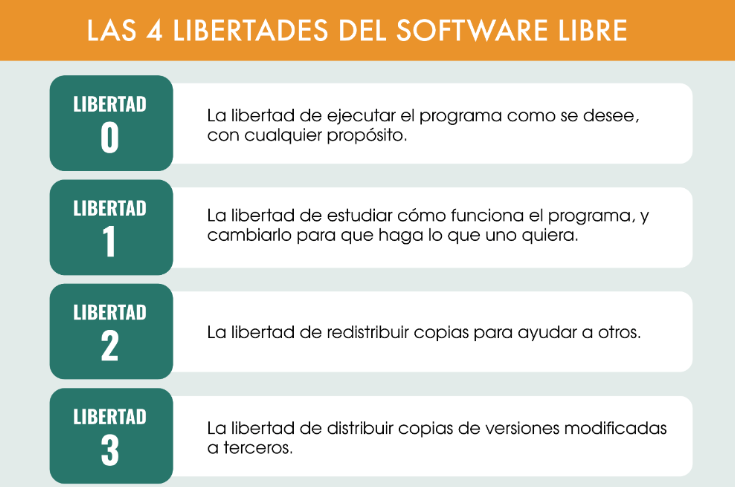
\includegraphics[width=1\linewidth, height=1
  \textheight]{libertades.png}
  \caption{Libertades}
  \label{fig:etiqueta}
\end{figure}

\section{Virtualización}

La virtualización es una tecnología que se puede usar para crear representaciones virtuales de servidores, almacenamiento, redes y otras máquinas físicas. El software virtual imita las funciones del hardware físico para ejecutar varias máquinas virtuales a la vez en una única máquina física. Las empresas recurren a la virtualización para utilizar sus recursos de hardware de manera eficiente y obtener retornos mayores de sus inversiones. También potencia los servicios de computación en la nube que ayudan a las organizaciones a administrar la infraestructura de manera más eficaz. Las tecnologías de virtualización tuvieron su auge entre 2000 y 2010.

\vspace{5pt}
Vn sistema computacional se divide lógicamente en varias VM, cada una con un S.O diferente.

\vspace{5pt}
Ventajas: 
\begin{itemize}
    \item Disminuye costos de inversión de hardware .
    \item Disminuye el tiempo de experimentación o pruebas.
    \item Disminuye los costes de energía.

\vspace{5pt}
Ejemplos de plataformas de Virtualización:
    \item VMware
    \item Virtual Box
    \item KUM
    \item Virtuoso
    \item VirtualPc

VirtualBox: Es una  plataforma de gestión de virtual machines que sirve para crear, borrar, configurar, clonar, etc.
\end{itemize}

\section{Tipos de S.O}
\begin{itemize}
    \item Arquitectura Monolítica: todos los procesos se ejecutan en la sección de kernel

    \item Arquitectura de micro-kernel: está repartida por módulos. Si un módulo se colapsa, el resto del sistema sigue en funcionamiento
\end{itemize}

\section{Video}
\begin{itemize}
    \item Es importante confiar en uno mismo
    \item Los habitos, actitudes, comportamientos, etc, es la zona de confort.
    \item La zona de aprendizaje es para crecer como persona en cualqquier ámbito.
    \item La zona de panico o la zona de no experiencia se refiere a un momento donde no se quiere entrar.
    \item Si gestionamos los miedos nuestra autoestima crece y podemos cumplir los objetivos propuestos de una manera más llevadera.

\end{itemize}

\section{Features of operating system}
\subsection{Tipos de Kernel}

Está encargado de todas las funciones de mayor relevancia del hardware, sin importar cuál sea el sistema operativo, Linux, macOS, Windows, servidores, virtualizaciones como KVM, hasta tu smartphone tiene un Kernel en el núcleo que permite que abras WhatsApp. Curioso, ¿no? Está ahí y muchas veces no lo sabemos.

\begin{itemize}
    \item Kernel monolítico: es un Kernel de gran tamaño que puede gestionar todas las tareas. Se encarga de la gestión de memoria y procesos, así como de la comunicación entre los procesos y el soporte de las diferentes funciones de los drivers y el hardware. Los sistemas operativos que recurren al Kernel monolítico son Linux, OS X y Windows.
    \item Microkernel: los Kernel que están diseñados con pequeños tamaños tienen una clara función: evitar el colapso total del sistema en caso de un fallo. Para cumplir con todas las tareas como un Kernel monolítico cuenta con diferentes módulos. Es curioso, pero hasta ahora solo el Mach de OS X es el único que utiliza el microkernel.
    \item Kernel híbrido: combinación entre el microkernel y el Kernel monolítico. Nos encontramos ante un Kernel grande, pero compacto y que puede ser modulado y otras partes del mismo Kernel pueden cargarse de manera dinámica. Es utilizado en Linux y OS X. 

\end{itemize}

\subsection{Arquitectura Android}
Android es un sistema operativo móvil desarrollado por Google. Desde su lanzamiento en 2008, se ha convertido en uno de los sistemas operativos móviles más populares del mundo, con una gran cantidad de dispositivos que ejecutan Android en todo el mundo.
La arquitectura de Android se basa en un sistema operativo Linux y está compuesta por varias capas y componentes que trabajan juntos para proporcionar la funcionalidad del sistema. Estas capas incluyen la capa de aplicaciones, la capa de marco de trabajo, la capa de bibliotecas y la capa de kernel. La capa de aplicaciones alberga las aplicaciones instaladas, mientras que el kernel se encarga de administrar los recursos del hardware.

\subsection{Arquitectura IOS}
La arquitectura de iOS se compone de cuatro capas principales: Cocoa Touch Layer, Media Layer, Core Services Layer, Core OS Layer y Kernel and Device Drivers. Estas capas trabajan juntas para proporcionar un entorno operativo completo y eficiente, permitiendo a los desarrolladores crear aplicaciones de alta calidad para dispositivos Apple. La integración estrecha entre hardware y software es una característica distintiva de la arquitectura de iOS, lo que contribuye a la experiencia de usuario ya que su interfaz grafica es intuitiva, al igual que la seguridad de servicio de almacenamiento que proporciona. 

\subsection{Arquitectura MacOs}
El sistema operativo macOS está basado en el kernel de Darwin, que a su vez se basa en UNIX. Esto ha sido una gran ventaja para muchos desarrolladores que aprecian la estabilidad y confiabilidad de UNIX, el sistema operativo macOS es mucho más complejo en su totalidad. Darwin es la base del sistema operativo macOS actual. Aunque Darwin es de código abierto, la última versión es macOs Ventura la cual se lanzó al público en octubre de 2022. Es importante destacar que Darwin es un sistema operativo sin interfaz gráfica de usuario.

\vspace{5pt}

\newpage
\section{Clasificación de los Sistemas Operativos}
Existen diferentes tipos de sistemas operativos, como por ejemplo: 
\begin{itemize}
      \item\textbf{Sistema operativo de lote simple:} Administra y ejecuta tareas simples en lotes sin interacción del usuario.
      \item \textbf{Sistema operativo de multiprogramación en lote:} Permite la ejecución simultánea de múltiples programas en lotes, mejorando la utilización del CPU.
      \item \textbf{Sistema operativo de tiempo compartido:} Permite el uso compartido de recursos y la ejecución simultánea de múltiples tareas para múltiples usuarios.
      \item \textbf{Sistema operativo de multiprocesador:} Administra y coordina eficientemente múltiples procesadores en un solo sistema.
      \item \textbf{Sistema operativo distribuido:} Permite que múltiples computadoras se comuniquen y trabajen juntas como un solo sistema coherente.
      \item \textbf{Sistema operativo de red:} Proporciona servicios y funcionalidades para la gestión de recursos y comunicación en una red de computadoras.
      \item \textbf{Sistema operativo en tiempo real:} Proporciona una respuesta en tiempo real predecible y rápida para aplicaciones críticas y sensibles al tiempo.
      \item \textbf{Sistema operativo móvil:} Proporciona un entorno operativo para dispositivos móviles, como teléfonos inteligentes y tabletas, con características y funcionalidades específicas para su uso portátil.
  \end{itemize}
  
\vspace{5pt}

\begin{figure}[htb]
  \centering
  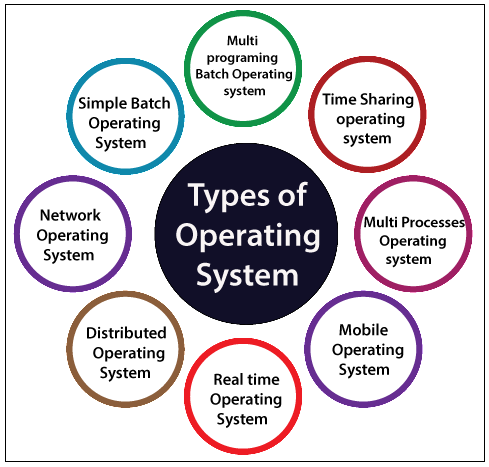
\includegraphics[width=0.8\linewidth]{introduccion/Types-of-OS.png}
  \caption{Tipos de sistemas operativos}
  \footnotesize Fuente: \url{https://windowscult.com/operating-system/}
  \label{fig:etiqueta}
\end{figure}
\newpage
\subsection{Sistemas de archivos linux}
Los sistemas de archivos son la forma en que los sistemas operativos organizan y almacenan los datos en un disco duro u otro medio de almacenamiento. Proporcionan una estructura jerárquica para organizar y acceder a los archivos y directorios.

\begin{itemize}

\item \textbf{FAT32}: Utilizado principalmente en dispositivos USB y tarjetas de memoria, es compatible con la mayoría de los sistemas operativos, pero tiene limitaciones en el tamaño de archivo y partición.

\item \textbf{NTFS}: Utilizado en Windows, es más avanzado y ofrece características como permisos de archivo, compresión y encriptación.

\item \textbf{Ext4}: Utilizado en Linux, ofrece mejor rendimiento y confiabilidad que sus predecesores, con soporte para tamaños de archivo y partición más grandes.

\item \textbf{APFS}: Utilizado en macOS y iOS, ofrece eficiencia, seguridad y compatibilidad con características como instantáneas, encriptación y administración de espacio libre.

\item \textbf{HFS}: Utilizado en versiones anteriores de macOS, ahora está siendo reemplazado por APFS, pero aún se encuentra en uso en algunos sistemas.

\item\textbf{ZFS}: Utilizado en sistemas operativos basados en Unix, ofrece integridad de datos, administración avanzada de almacenamiento y capacidad para manejar grandes volúmenes de datos.
    
\end{itemize}

\section{Reflexion}
Diego Medina Naranjo, sus miedos le ganaron y no gano sus oportunidades.
Libro: El poder invisible del amor.
Juan 14,6. Jesucristo dijo: "Yo soy el camino, la verdad y la vida. Nadie viene al Padre si no es por mi.

\section{Tipos de kerner}
Kernel controla todos los accesos al procesador y la memoria, pero también es responsable de los drivers (controladores) más importantes y tiene la capacidad de acceder a los hardwares de forma directa. Kernel es basado en Linux.

\begin{itemize}

\item \textbf{Kernel monolítico:}: es un Kernel de gran tamaño que puede gestionar todas las tareas. Se encarga de la gestión de memoria y procesos, así como de la comunicación entre los procesos y el soporte de las diferentes funciones de los drivers y el hardware. Los sistemas operativos que recurren al Kernel monolítico son Linux, OS X y Windows.

\item \textbf{Microkernel:}: los Kernel que están diseñados con pequeños tamaños tienen una clara función: evitar el colapso total del sistema en caso de un fallo. Para cumplir con todas las tareas como un Kernel monolítico cuenta con diferentes módulos. Es curioso, pero hasta ahora solo el Mach de OS X es el único que utiliza el microkernel.

\item \textbf{Kernel híbrido}: combinación entre el microkernel y el Kernel monolítico. Nos encontramos ante un Kernel grande, pero compacto y que puede ser modulado y otras partes del mismo Kernel pueden cargarse de manera dinámica. Es utilizado en Linux y OS X. 

\end{itemize}

\vspace{5pt}

\begin{figure}[htb]
  \centering
  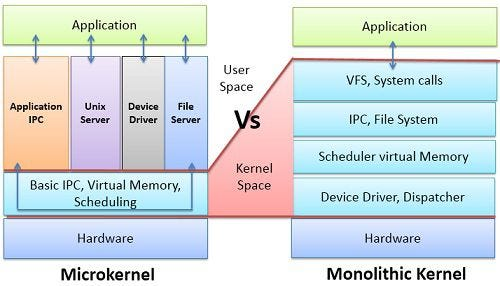
\includegraphics[width=1\linewidth]{TK.png}
  \caption{Tipos de Kernel}
  \label{fig:etiqueta}
\end{figure}

\subsection{¿Qué es IPC?}
La comunicación entre procesos (comúnmente IPC, del inglés Inter-Process Communication) es una función básica de los sistemas operativos. Los procesos pueden comunicarse entre sí a través de compartir espacios de memoria, ya sean variables compartidas o buffers, o a través de las herramientas provistas por las rutinas de IPC. La IPC provee un mecanismo que permite a los procesos comunicarse y sincronizarse entre sí, normalmente a través de un sistema de bajo nivel de paso de mensajes que ofrece la red subyacente.

\section{Video Steve Jobs}
Dejo la universidad, su madre biologíca lo dio en adopción, se salio de la universidad porque no le veía sentido y se estaba gastando los ahorros de toda la vida de sus padres y prefierio no entrar a clases que no le interesaban ya que sentía que no le iba a ayudar a descubrir lo que quería en la vida. No puedes conectar los puntos hacia adelante, solamente hacia atrás, y tener la confianza de que en algun momento esos puntos se uniran. Creo PIXAR, conocio a su esposa. Frase de vida: sigue hambriento sigue alocado. 1955-2011

\section{Tipos de Sistemas Operativos}
\subsection{VFS}
La interfaz del sistema de archivos virtual (VFS), también conocida como interfaz v-node, proporciona un puente entre los sistemas de archivos físicos y lógicos. La información siguiente describe la interfaz del sistema de archivos virtual, sus estructuras de datos y sus archivos de cabecera, y explica cómo configurar un sistema de archivos virtual.

\subsection{Open Source Software}
El software open source se lanza con una licencia específica que pone su código fuente a disposición de los usuarios finales de forma legal. Hay muchas licencias de este tipo, pero normalmente el software se considera open source si cumple con las siguientes condiciones:

\begin{itemize}

\item  Está disponible en forma de código fuente sin costo adicional, lo cual significa que los usuarios pueden visualizar el código del software y hacer todos los cambios que deseen.

\item El código fuente se puede reutilizar en un software nuevo, así que cualquier persona puede usar el código fuente para desarrollar su propio programa y distribuirlo.

\end{itemize}

\subsection{Biografía de Steve Jobs}

Steve Paul Jobs nació el 24 de febrero de 1955 en San Francisco y falleció el 5 de octubre de 2011 en Palo Alto, California. Fue un empresario, diseñador industrial y magnate empresarial estadounidense, conocido por su papel en la fundación de Apple Inc. y su contribución a la revolución de la industria tecnológica.

\subsection*{Logros más importantes}

\begin{quote}
\begin{itemize}
    \item \textbf{Apple y la revolución tecnológica:} Jobs fue el padre del primer ordenador personal y fundador de Apple Computer, una de las empresas más innovadoras del sector. Revolucionó los mercados de los ordenadores personales, la telefonía móvil y la música digital durante más de tres décadas.
    
    \item \textbf{Productos icónicos:} Bajo su liderazgo, Apple lanzó productos icónicos como el Macintosh, el iPod, el iPhone y el iPad, que transformaron la forma en que interactuamos con la tecnología.
    
    \item \textbf{Innovación y visión:} Se caracterizó por tener ideas visionarias en el campo de la tecnología, lo que le llevó a revolucionar la industria a través de sus productos.
\end{itemize}
\end{quote}

Steve Jobs fue un visionario que dejó un legado duradero en la industria tecnológica, transformando la forma en que interactuamos con la tecnología y dejando una huella imborrable en el mundo moderno.
\begin{figure}[htb]
  \centering
  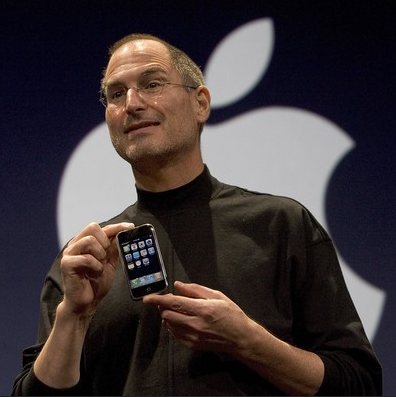
\includegraphics[width=0.8\linewidth]{bibliografias/jobs.PNG}
  \caption{Steve Jobs presentando el IPhone}
  \label{fig:etiqueta}
\end{figure}

\newpage

\subsection{Biografía de Bill Gates}
Bill Gates, nació el 28 de octubre de 1955 en Seattle, Washington, Estados Unidos es un empresario y filántropo estadounidense conocido por ser el cofundador de Microsoft Corporation y por su labor en la Fundación Bill y Melinda Gates. 
\subsection*{Aspectos importantes de su vida y carrera}
\begin{quote}
\begin{itemize}
\item En 1975, Gates cofundó Microsoft junto a su amigo Paul Allen.
\item Bajo el liderazgo de Gates, Microsoft se convirtió en la empresa de software para computadoras personales más grande del mundo.
\item En 2008, Gates dejó su cargo ejecutivo en Microsoft para dedicarse a tiempo completo a la Fundación Bill y Melinda Gates, la cual se enfoca en abordar problemas globales de salud y desarrollo.
\item Gates ha recibido numerosos premios y reconocimientos a lo largo de su carrera, incluyendo la Medalla Presidencial de la Libertad en 2016.
\item Ha realizado predicciones sobre el futuro de la tecnología y ha escrito libros sobre negocios y tecnología, como "Negocios a la velocidad del pensamiento"
\end{itemize}
\end{quote}

\begin{figure}[htb]
  \centering
  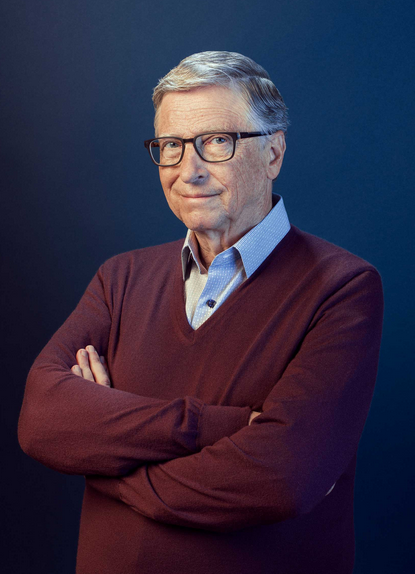
\includegraphics[width=0.5\linewidth]{bibliografias/gates.PNG}
  \caption{Bill Gates.}
  \label{fig:etiqueta}
\end{figure}
\newpage

\section{Conceptos clave - Acrónimos}
\begin{itemize}
    \item GNU - GNU is not Unix
    \item GCC - GNU C Compiler
    \item GPL - GNU Public License
    \item FSF - Free Software Foundation
    \item BASH - Bourne Again Shell
    \item FAT - File Allocation Table
    \item NTFS - New Technology File System
    \item CLI - Command Line Interface
    \item IBC - International Business Machines
    \item UNIX - Uniplex Information and Computing System
    \item IPC - Inter-Process Communication
    \item DDL - Data Definition Language
    \item DVM - Dalvik Virtual Machine (Máquina virtual de Android)
    \item GUI - Graphical User Interface
    \item XNU - X is Not Unix
    \item MAC - Macintosh
    \item HDD - Hard Disk Drive
    \item SSD - Solid State Drive
    \item VFS - Virtual File System
    \item EXT3 - Third Extended Filesystem
    \item HPFS - High Performance File System
    \item VFAT - Virtual File Allocation Table
    \item EXT4 - Fourth Extended Filesystem
    \item FreeBSD - Free Berkeley Software Distribution
    \item EMACS - Editor MACroS
    \item WINDOWS NT - Windows New Technology
\end{itemize} 

\section{Programación en Shell Script}

\subsection{Operadores de comparación}

-eq
es igual a

-ne
no es igual a / es distinto a

-gt
es mayor que

-ge
es mayor que o igual a

-lt
es menor que

-le
es menor que o igual a

<
es menor que (dentro de doble paréntesis)

<=
es menor que o igual a (dentro de doble paréntesis)

>
es mayor que (dentro de doble paréntesis)

>=
es mayor que o igual a (dentro de doble paréntesis)

Comparación de cadenas

=
es igual a

==
es igual a

\subsection{Ejercicio 1}
\begin{lstlisting}
#!/bin/bash
clear
echo "Ingrese el 1er numero";
read num1;
echo "Ingrese el 2do numero";
read num2;
if [ $num1 -lt $num2 ]; then
echo "el menor  numero es: $num1"
elif [ $num2 -lt $num1 ]; then
echo "El menor es: $num2";
else 
echo "$num1, $num2 son iguales";
fi
#I love linux
\end{lstlisting}
\begin{figure}
    \centering
    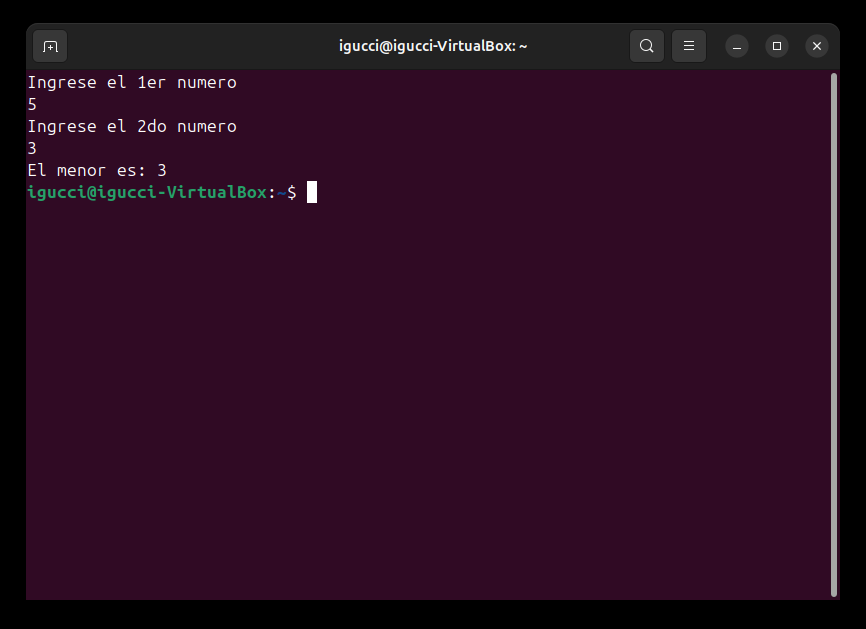
\includegraphics[width=0.5\linewidth]{Ej1.png}
    \caption{Ejercicio 1}
 
\end{figure}

\subsection{Ejercicio 2}
\begin{lstlisting}
#!/bin/bash

echo "Ingrese el primer número entero positivo:"
read num1

echo "Ingrese el segundo número entero positivo:"
read num2

suma=$(expr $num1 + $num2)
resta=$(expr $num1 - $num2)
multiplicacion=$(expr $num1 \* $num2)
division=$(expr $num1 / $num2)

echo "Resultados:"
echo "Suma: $num1 + $num2 = $suma"
echo "Resta: $num1 - $num2 = $resta"
echo "Multiplicación: $num1 * $num2 = $multiplicacion"
echo "División: $num1 / $num2 = $division"
\end{lstlisting}

\begin{figure}
    \centering
    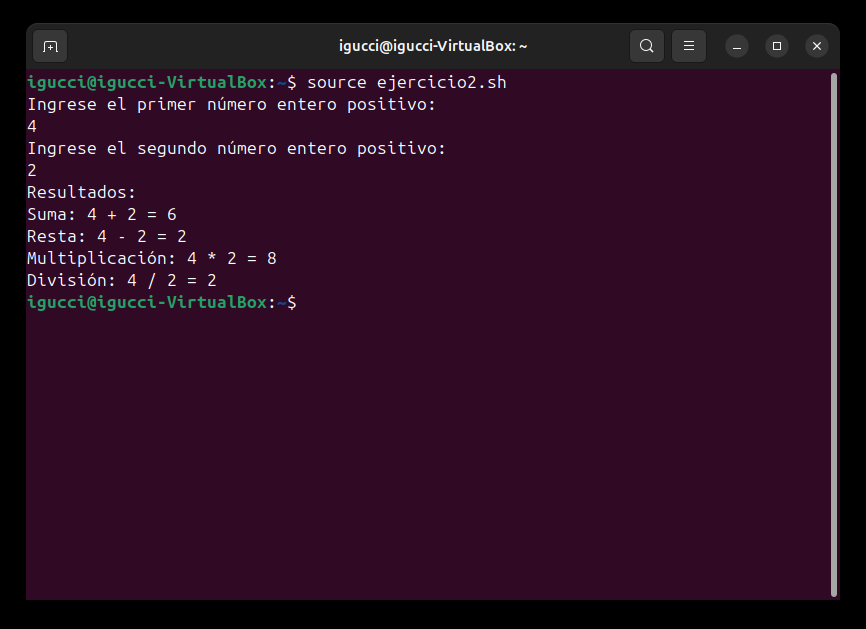
\includegraphics[width=0.5\linewidth]{Ej2.png}
    \caption{Ejercicio 2}

\end{figure}

\subsection{Ejercicio 3}
\begin{lstlisting}
#!/bin/bash
cont=0
while [ $cont -lt 11 ]
do
echo $cont
cont=$((cont + 1))
done
# I LOVE LINUX
\end{lstlisting}
\begin{figure}
    \centering
    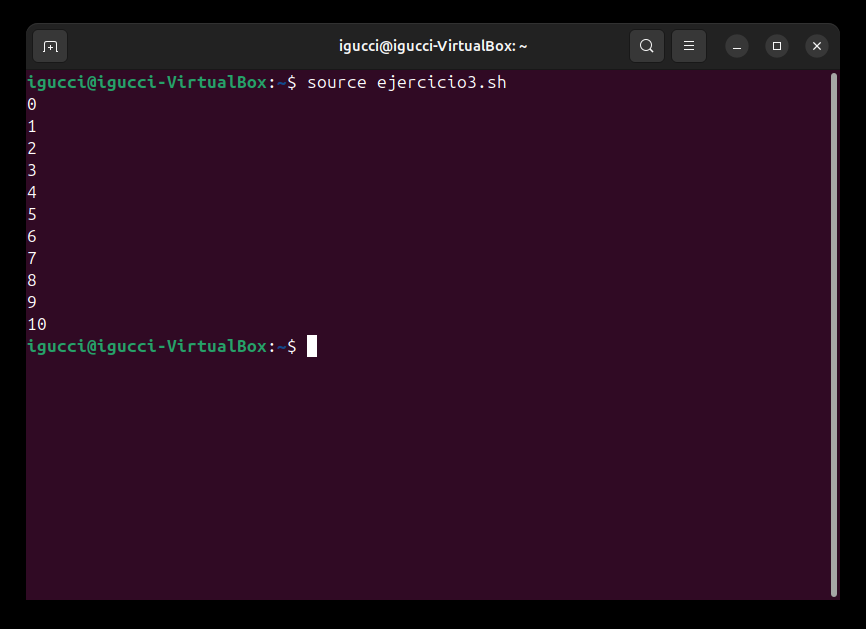
\includegraphics[width=0.5\linewidth]{Ej3.png}
    \caption{Ejercicio 3}

\end{figure}


\subsection{Ejercicio 4}
\begin{lstlisting}
#!/bin/bash

# Imprimir los primeros 20 múltiplos de 3
echo "Los primeros 20 múltiplos de 3 son:"
for (( i=1; i<=20; i++ )); do
  multiplo=$((i * 3))
  echo $multiplo
done

\end{lstlisting}
\begin{figure}
    \centering
    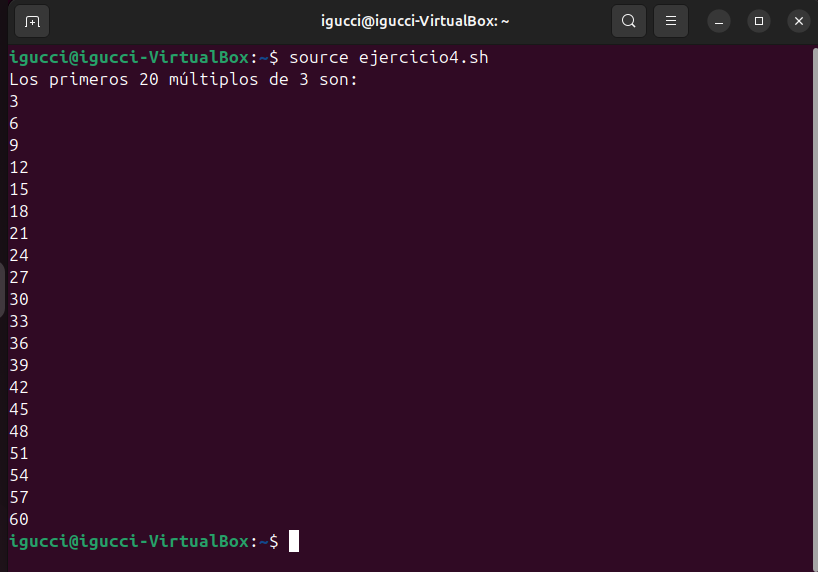
\includegraphics[width=0.5\linewidth]{Ej4.png}
    \caption{Ejercicio 4}

\end{figure}

\subsection{Ejercicio 5}
\begin{lstlisting}
#!/bin/bash

# Leer un número entero positivo
echo "Ingrese un número entero positivo:"
read num

# Calcular y mostrar la tabla de multiplicar hasta el 20
for ((i = 1; i <= 20; i++)); do
  resultado=$((num * i))
  echo "$num x $i = $resultado"
done
\end{lstlisting}

\begin{figure}
    \centering
    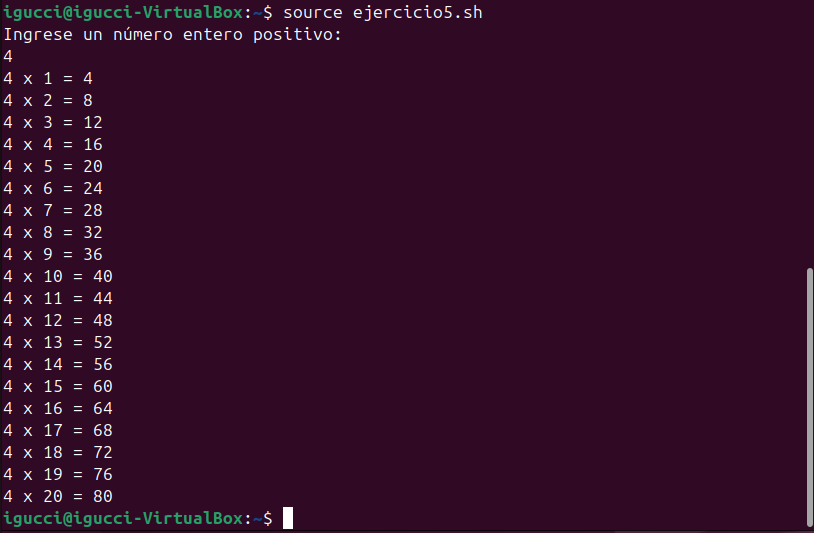
\includegraphics[width=0.5\linewidth]{Ej5.png}
    \caption{Ejercicio 5}

\end{figure}

\section{Proceso de Arranque en Linux}

\begin{itemize}
\item BIOS  -  Basic Input/ Output System - post Power on self test - Codigo de Arranque
\item MBR -  Master Boot Record - Codigo de Arranque (446 bytes) - Tabla de particiones (64 bytes)  - Firma del HDD (12 bytes)
\item GRUB - Grand Unified Boot loader - Gestor de Arranque, Menu de Opciones - Ejecutar el Kernel
\item KERNEL - Archivo comp que tiene el nucleo del S.O - Se ejecuta en la RAM 
\item INIT - Descomprime y activa las aplicaciones y servicios - Interc el filesystem 
\item RUN LEVEL 

\end{itemize}

\begin{figure}
    \centering
    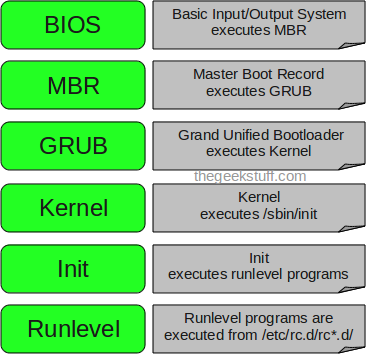
\includegraphics[width=0.5\linewidth]{PAL.png}
    \caption{Proceso de Arranque}
\end{figure}

\section{Basic Calculator}

\begin{figure}
    \centering
    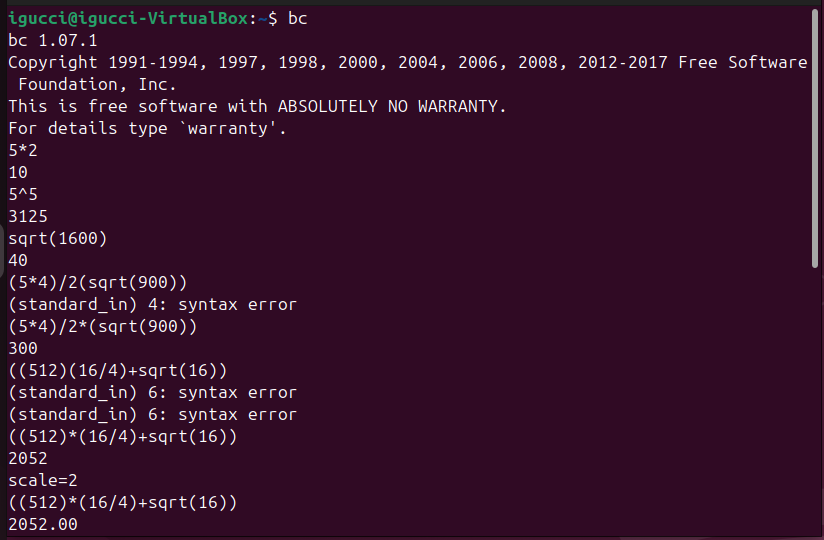
\includegraphics[width=1
    \linewidth]{bc1.png}
    \caption{BC }
\end{figure}
\begin{figure}
    \centering
    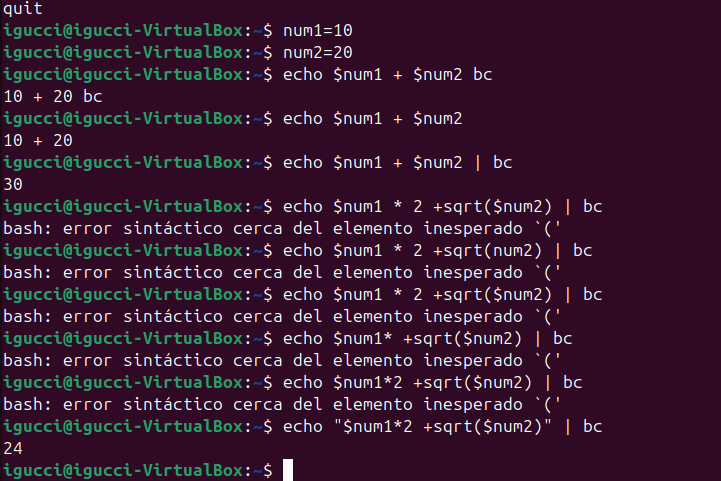
\includegraphics[width=1\linewidth]{bc2.png}
    \caption{BC2}
\end{figure}
\begin{figure}
    \centering
    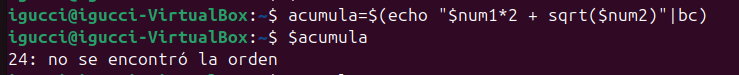
\includegraphics[width=1\linewidth]{BC3.png}
    \caption{BC3}
\end{figure}
\subsection{Ejercicio1}
Que imprima los 10 multiplos de 5, utilizando bc con 2 decimales
\begin{lstlisting}
#!/bin/bash
#Author: Gustavo Aguas
#Date" 05 Jun 2024

i=1

while [ $i -le 10 ]
do
    
    multiplo=$(echo "scale=2; 5 * $i" | bc)

    
    echo "Múltiplo $i de 5: $multiplo"

    
    i=$((i + 1))
done
echo I LOVE LINUX
\end{lstlisting}
\begin{figure}
    \centering
    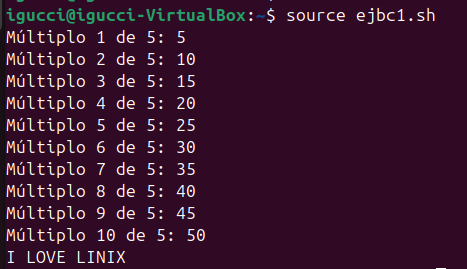
\includegraphics[width=1\linewidth]{ejbc1.png}
    \caption{EJ1}
\end{figure}

\subsection{Ejercicio2}
Que lea un numero ingresado por teclado y muestre la tabla de multiplicar del numero hasta el 20.
\begin{lstlisting}
#!/bin/bash
#Author: Gustavo Aguas
#Date" 05 Jun 2024
read -p "Ingrese un número: " numero


if ! [[ $numero =~ ^[0-9]+(\.[0-9]+)?$ ]]; then
    echo "Error: '$numero' no es un número válido."
    exit 1
fi


echo "Tabla de multiplicar del número $numero hasta el 20:"
for ((i = 1; i <= 20; i++)); do
    resultado=$(echo "scale=2; $numero * $i" | bc)
    echo "$numero x $i = $resultado"
done
echo I LOVE LINUX

\end{lstlisting}
\begin{figure}
    \centering
    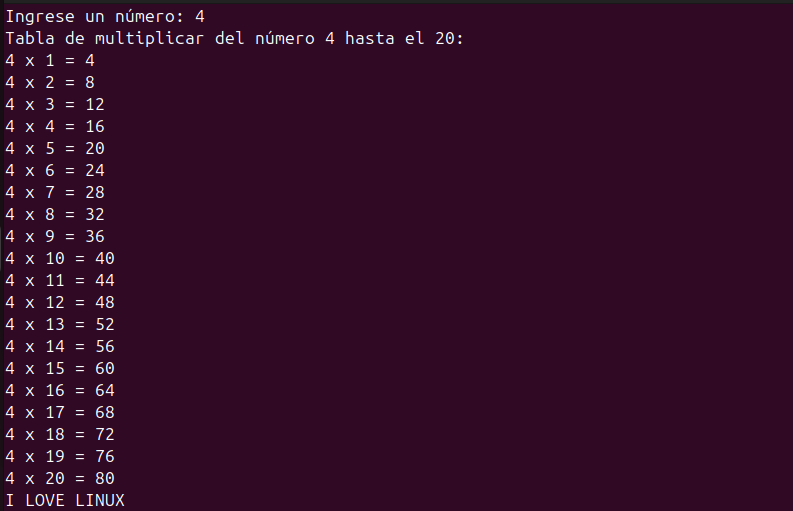
\includegraphics[width=1\linewidth]{ej2bc.png}
    \caption{Ej2}
\end{figure}

\subsection{Ejercicio3}
Que llame a una funcion que calcule el factorial de un numero ingresado, usando bc.
\begin{lstlisting}
#!/bin/bash
#Author: Gustavo Aguas
#Date" 05 Jun 2024

factorial() {
    
    if ! [[ $1 =~ ^[1-9][0-9]*$ ]]; then
        echo "Error: '$1' no es un número entero positivo válido."
        return 1
    fi

  
    resultado=1

    # Calcular el factorial
    for ((i = 1; i <= $1; i++)); do
        resultado=$(echo "scale=0; $resultado * $i" | bc)
    done

   
    echo "El factorial de $1 es: $resultado"
}

read -p "Ingrese un número entero positivo para calcular su factorial: " numero

factorial "$numero"

echo I LOVE LINUX

\end{lstlisting}
\begin{figure}
    \centering
    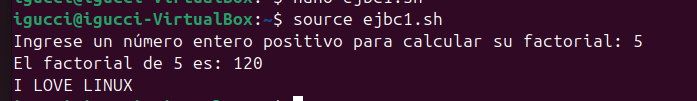
\includegraphics[width=1\linewidth]{ej3bc.png}
    \caption{EJ 3}
\end{figure}

\subsection{Ejercicio4}

Es una secuencia de numeros que sigue una regla especifica 

serie1: 2,5,8,11,14... Serie Aritmetica
serie2: 3,6,12,24 ...  Serie Geometrica 
serie3: 0,1,1,2,3,5,8 ...  Serie de Fibonacci
\begin{lstlisting}
#!/bin/bash
#Author: Gustavo Aguas
#Date" 05 Jun 2024

factorial() {
    
    if ! [[ $1 =~ ^[1-9][0-9]*$ ]]; then
        echo "Error: '$1' no es un número entero positivo válido."
        return 1
    fi

  
    resultado=1

    # Calcular el factorial
    for ((i = 1; i <= $1; i++)); do
        resultado=$(echo "scale=0; $resultado * $i" | bc)
    done

   
    echo "El factorial de $1 es: $resultado"
}

read -p "Ingrese un número entero positivo para calcular su factorial: " numero

factorial "$numero"

echo I LOVE LINUX

\end{lstlisting}

\section{Repaso Prueba}
Estrategias de aprendizaje para la preparación del Examen

\subsection{Parte Teórica}

\subsubsection{1. Elaborar un listado de acronimos en orden alfabetico}

\begin{itemize}
   \item BASH - Bourne Again Shell
\item BIOS - Basic Input/Output System
\item CLI - Command Line Interface
\item CPU - Central Processing Unit
\item DDL - Data Definition Language
\item DHCP - Dynamic Host Configuration Protocol
\item DNS - Domain Name System
\item DOS - Disk Operating System
\item DVM - Dalvik Virtual Machine (Máquina virtual de Android)
\item EFI - Extensible Firmware Interface
\item EMACS - Editor MACroS
\item EXT3 - Third Extended Filesystem
\item EXT4 - Fourth Extended Filesystem
\item FAT - File Allocation Table
\item FTP - File Transfer Protocol
\item FreeBSD - Free Berkeley Software Distribution
\item FSF - Free Software Foundation
\item GCC - GNU C Compiler
\item GIMP - GNU Image Manipulation Program
\item GNU - GNU is not Unix
\item GPL - GNU Public License
\item GRUB - GRand Unified Bootloader
\item GUI - Graphical User Interface
\item HDD - Hard Disk Drive
\item HPFS - High Performance File System
\item HTTP - Hypertext Transfer Protocol
\item HTTPS - Hypertext Transfer Protocol Secure
\item IBM - International Business Machines
\item IPC - Inter-Process Communication
\item IP - Internet Protocol
\item ISP - Internet Service Provider
\item LTS - Long Term Support
\item MAC - Media Access Control
\item MBR - Master Boot Record
\item NAT - Network Address Translation
\item NTFS - New Technology File System
\item OS - Operating System
\item POST - Power-On Self Test
\item POSIX - Portable Operating System Interface
\item RAM - Random Access Memory
\item ROM - Read-Only Memory
\item SATA - Serial Advanced Technology Attachment
\item SCSI - Small Computer System Interface
\item SSD - Solid State Drive
\item SSH - Secure Shell
\item TCP - Transmission Control Protocol
\item UEFI - Unified Extensible Firmware Interface
\item UDP - User Datagram Protocol
\item UNIX - Uniplex Information and Computing System
\item URL - Uniform Resource Locator
\item VFAT - Virtual File Allocation Table
\item VFS - Virtual File System
\item VM - Virtual Machine
\item VPN - Virtual Private Network
\item WINDOWS NT - Windows New Technology
\item XNU - X is Not Unix
\item XORG - X Window System
\item XML - Extensible Markup Language
\item YAML - YAML Ain't Markup Language
\item ZIP - Zone Information Protocol
\end{itemize} 

\subsubsection{2. Preguntas con respuestas cortas}
\begin{enumerate}[label=\textbf{\arabic*.}, leftmargin=2cm]

    \item ¿Cuándo se liberó Linux? 
    \begin{itemize}
        \item 1991
    \end{itemize}

    \item ¿Cuál es el sistema operativo base de Mac? 
    \begin{itemize}
        \item Unix
    \end{itemize}

    \item ¿Qué significa la sigla OS? 
    \begin{itemize}
        \item Operating System
    \end{itemize}

    \item ¿Qué es un kernel? 
    \begin{itemize}
        \item Núcleo
    \end{itemize}

    \item ¿Qué tipo de kernel usa Linux? 
    \begin{itemize}
        \item Monolítico
    \end{itemize}

    \item ¿Cuál es el sistema de archivos por defecto de Windows? 
    \begin{itemize}
        \item NTFS
    \end{itemize}

    \item ¿Qué significa la sigla RAM? 
    \begin{itemize}
        \item Random Access Memory
    \end{itemize}

    \item ¿Qué significa la sigla ROM? 
    \begin{itemize}
        \item Read-Only Memory
    \end{itemize}

    \item ¿Qué significa BIOS? 
    \begin{itemize}
        \item Basic Input/Output System
    \end{itemize}

    \item ¿Qué es UEFI? 
    \begin{itemize}
        \item Firmware
    \end{itemize}

    \item ¿Qué sistema de archivos usa Linux por defecto? 
    \begin{itemize}
        \item EXT4
    \end{itemize}

    \item ¿Qué es un proceso en un sistema operativo? 
    \begin{itemize}
        \item Programa
    \end{itemize}

    \item ¿Qué protocolo se usa para la transferencia de archivos? 
    \begin{itemize}
        \item FTP
    \end{itemize}

    \item ¿Qué significa SSH? 
    \begin{itemize}
        \item Secure Shell
    \end{itemize}

    \item ¿Qué tipo de sistema operativo es Windows? 
    \begin{itemize}
        \item Privativo
    \end{itemize}

    \item ¿Qué significa POSIX? 
    \begin{itemize}
        \item Portable Operating System Interface
    \end{itemize}

    \item ¿Qué hace el comando `ls` en Unix/Linux? 
    \begin{itemize}
        \item Listar
    \end{itemize}

    \item ¿Qué comando se usa para cambiar de directorio en Unix/Linux? 
    \begin{itemize}
        \item cd
    \end{itemize}

    \item ¿Qué sistema operativo utiliza el kernel XNU? 
    \begin{itemize}
        \item macOS
    \end{itemize}

    \item ¿Cuál es el sistema de ventanas más común en Linux? 
    \begin{itemize}
        \item Xorg
    \end{itemize}

    \item ¿Qué es un hipervisor? 
    \begin{itemize}
        \item Virtualización
    \end{itemize}

    \item ¿Qué herramienta se usa para el arranque de sistemas operativos en Linux? 
    \begin{itemize}
        \item GRUB
    \end{itemize}

    \item ¿Cuál es el sistema operativo móvil desarrollado por Google? 
    \begin{itemize}
        \item Android
    \end{itemize}

    \item ¿Qué comando se usa para copiar archivos en Unix/Linux? 
    \begin{itemize}
        \item cp
    \end{itemize}

    \item ¿Qué sistema operativo fue desarrollado por Bell Labs? 
    \begin{itemize}
        \item Unix
    \end{itemize}

\end{enumerate}


\subsubsection{3. Preguntas de opción simple }

\begin{enumerate}[label=\textbf{\arabic*.}, leftmargin=2cm]

    \item ¿Cuál es el comando de Linux que muestra el contenido de un archivo?
    \begin{enumerate}[label=\Alph*.]
        \item cat
        \item ls
        \item grep
        \item \textbf{more*}
        \item head
    \end{enumerate}

    \item ¿Qué comando se utiliza para cambiar al directorio padre en Linux?
    \begin{enumerate}[label=\Alph*.]
        \item cd ..
        \item \textbf{cd ..*}
        \item cd /
        \item cd ~
        \item cd -
    \end{enumerate}

    \item ¿Cuál es el comando para crear un enlace simbólico en Linux?
    \begin{enumerate}[label=\Alph*.]
        \item  \textbf {ln -s*}
        \item link
        \item sym
        \item softlink
        \item sl
    \end{enumerate}

    \item ¿Qué comando se utiliza para mostrar la fecha y hora actual en Linux?
    \begin{enumerate}[label=\Alph*.]
        \item \textbf{date*}
        \item time
        \item clock
        \item datetime
        \item now
    \end{enumerate}

    \item ¿Cuál es el comando para cambiar el nombre de un archivo en Linux?
    \begin{enumerate}[label=\Alph*.]
        \item rename
        \item ren
        \item \textbf{mv*}
        \item change
        \item mvn
    \end{enumerate}

    \item ¿Qué comando se utiliza para buscar texto dentro de archivos en Linux?
    \begin{enumerate}[label=\Alph*.]
        \item find
        \item \textbf{grep*}
        \item search
        \item locate
        \item textsearch
    \end{enumerate}

    \item ¿Cuál es el comando para detener la ejecución de un proceso en Linux?
    \begin{enumerate}[label=\Alph*.]
        \item kill
        \item stop
        \item terminate
        \item end
        \item \textbf{kill*}
    \end{enumerate}

    \item ¿Qué comando se utiliza para ver el contenido de un archivo en orden inverso en Linux?
    \begin{enumerate}[label=\Alph*.]
        \item more
        \item tail
        \item reverse
        \item \textbf{tac*}
        \item rev
    \end{enumerate}

    \item ¿Cuál es el comando para eliminar un directorio y su contenido en Linux?
    \begin{enumerate}[label=\Alph*.]
        \item rmdir
        \item rm -f
        \item \textbf{rm -rf*}
        \item deltree
        \item removedir
    \end{enumerate}

    \item ¿Qué comando se utiliza para mostrar el espacio utilizado y disponible en el sistema de archivos en Linux?
    \begin{enumerate}[label=\Alph*.]
        \item space
        \item \textbf{df*}
        \item usage
        \item du
        \item disk
    \end{enumerate}

    \item ¿Cuál es el comando para cambiar los permisos de un archivo en Linux?
    \begin{enumerate}[label=\Alph*.]
        \item perm
        \item chperm
        \item \textbf{chmod*}
        \item chown
        \item chgrp
    \end{enumerate}

    \item ¿Qué comando se utiliza para buscar archivos por su nombre en Linux?
    \begin{enumerate}[label=\Alph*.]
        \item find
        \item search
        \item \textbf{locate*}
        \item grep
        \item filesearch
    \end{enumerate}

    \item ¿Cuál es el comando para comprimir archivos en Linux?
    \begin{enumerate}[label=\Alph*.]
        \item zip
        \item tar
        \item compress
        \item gzip
        \item \textbf{tar*}
    \end{enumerate}

    \item ¿Qué comando se utiliza para renombrar archivos de forma masiva en Linux?
    \begin{enumerate}[label=\Alph*.]
        \item rename
        \item mv
        \item \textbf{rename*}
        \item ren
        \item batchrename
    \end{enumerate}

    \item ¿Cuál es el comando de Linux que crea un archivo vacío?
    \begin{enumerate}[label=\Alph*.]
        \item cat
        \item more
        \item \textbf{touch*}
        \item todas son correctas
        \item ninguna es correcta
    \end{enumerate}

\end{enumerate}


4. Preguntas de selección múltiple

\begin{enumerate}
    \item ¿Cuáles son características de los sistemas operativos de código abierto?
    \begin{itemize}
        \item[\textbf{a.}] Costo elevado
        \item[\textbf{b.}] Acceso al código fuente
        \item[\textbf{c.}] Libertad para modificar y distribuir
        \item[\textbf{d.}] Soporte exclusivo de una empresa
    \end{itemize}
    Respuesta correcta: \textbf{b} y \textbf{c}.

    \item ¿Cuáles son algunas distribuciones populares de Linux?
    \begin{itemize}
        \item[\textbf{a.}] Ubuntu
        \item[\textbf{b.}] Fedora
        \item[\textbf{c.}] Windows
        \item[\textbf{d.}] CentOS
    \end{itemize}
    Respuesta correcta: \textbf{a}, \textbf{b}, y \textbf{d}.

    \item ¿Qué son las interfaces gráficas de usuario (GUI) en Linux?
    \begin{itemize}
        \item[\textbf{a.}] Entornos que permiten interacciones visuales con el sistema operativo
        \item[\textbf{b.}] Herramientas exclusivas para programadores
        \item[\textbf{c.}] Proporcionan ventanas, iconos y menús para facilitar el uso del sistema
        \item[\textbf{d.}] Componentes del kernel
    \end{itemize}
    Respuesta correcta: \textbf{a} y \textbf{c}.

    \item ¿Cuál es el propósito principal del comando `chmod` en Linux?
    \begin{itemize}
        \item[\textbf{a.}] Cambiar el propietario de un archivo
        \item[\textbf{b.}] Cambiar los permisos de acceso de un archivo
        \item[\textbf{c.}] Comprimir archivos
        \item[\textbf{d.}] Establecer permisos de lectura, escritura y ejecución
    \end{itemize}
    Respuesta correcta: \textbf{b} y \textbf{d}.

    \item ¿Cuál de los siguientes es un gestor de paquetes comúnmente utilizado en distribuciones basadas en Debian?
    \begin{itemize}
        \item[\textbf{a.}] apt-get
        \item[\textbf{b.}] pacman
        \item[\textbf{c.}] yum
        \item[\textbf{d.}] dnf
    \end{itemize}
    Respuesta correcta: \textbf{a}.

    \item ¿Cuál es la extensión comúnmente utilizada para los scripts de shell en Linux?
    \begin{itemize}
        \item[\textbf{a.}] .txt
        \item[\textbf{b.}] .sh
        \item[\textbf{c.}] .exe
        \item[\textbf{d.}] .bat
    \end{itemize}
    Respuesta correcta: \textbf{b}.

    \item ¿Qué hace el comando `grep` en Linux?
    \begin{itemize}
        \item[\textbf{a.}] Crea un nuevo directorio
        \item[\textbf{b.}] Busca patrones en archivos
        \item[\textbf{c.}] Cambia los permisos de archivos
        \item[\textbf{d.}] Filtra líneas de texto según patrones especificados
    \end{itemize}
    Respuesta correcta: \textbf{b} y \textbf{d}.

    \item ¿Qué significa el acrónimo "LTS" en el contexto de las versiones de Linux?
    \begin{itemize}
        \item[\textbf{a.}] Latest Technical Support
        \item[\textbf{b.}] Long Term Support
        \item[\textbf{c.}] Lightweight System
        \item[\textbf{d.}] Limited Time Service
    \end{itemize}
    Respuesta correcta: \textbf{b}.

    \item ¿Cuál es el comando de Linux que crea un archivo vacío?
    \begin{itemize}
        \item[\textbf{a.}] cat
        \item[\textbf{b.}] more
        \item[\textbf{c.}] touch
        \item[\textbf{d.}] todas son correctas
        \item[\textbf{e.}] ninguna es correcta
    \end{itemize}
    Respuesta correcta: \textbf{c}.

    \item ¿Qué comando se utiliza para listar el contenido de un directorio en Linux?
    \begin{itemize}
        \item[\textbf{a.}] ls
        \item[\textbf{b.}] cd
        \item[\textbf{c.}] dir
        \item[\textbf{d.}] show
    \end{itemize}
    Respuesta correcta: \textbf{a}.

    \item ¿Cuál es el comando de Linux para cambiar el directorio de trabajo?
    \begin{itemize}
        \item[\textbf{a.}] mv
        \item[\textbf{b.}] cp
        \item[\textbf{c.}] cd
        \item[\textbf{d.}] pwd
    \end{itemize}
    Respuesta correcta: \textbf{c}.

    \item ¿Qué comando se utiliza para eliminar un archivo en Linux?
    \begin{itemize}
        \item[\textbf{a.}] erase
        \item[\textbf{b.}] del
        \item[\textbf{c.}] rm
        \item[\textbf{d.}] delete
    \end{itemize}
    Respuesta correcta: \textbf{c}.

    \item ¿Cuál es la función del comando `tar` en Linux?
    \begin{itemize}
        \item[\textbf{a.}] Comprimir archivos
        \item[\textbf{b.}] Empaquetar archivos en un archivo de almacenamiento
        \item[\textbf{c.}] Cambiar los permisos de un archivo
        \item[\textbf{d.}] Extraer archivos de un archivo de almacenamiento
    \end{itemize}
    Respuesta correcta: \textbf{b}
    \end{enumerate}
\subsection{Parte Practica}
\subsubsection{Ejercicio 1}
\begin{lstlisting}
#!/bin/bash
# Program Ejercicio 1
# Authors: Gustavo Aguas 
# Explicacion del programa: Este programa calcula el area del circulo

calcular_area() {
    local radio=$radio
    local area=$(echo "scale=2; 3.1416 * $radio * $radio" | bc)
    echo "$area"
}

echo "Ingrese el radio del círculo:"
read radio

resultado=$(calcular_area)
echo "El área del círculo con radio $radio es: $resultado"

# I love Linux
\end{lstlisting}
\begin{figure}
    \centering
    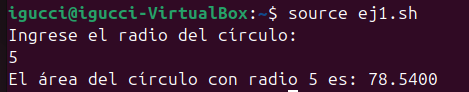
\includegraphics[width=1\linewidth]{Ejarea.png}
    \caption{Ej1. Area Círculo}
\end{figure}

\newpage
\subsubsection{Ejercicio 2}
\begin{lstlisting}
#!/bin/bash
# Program Ejercicio 2
# Authors: Gustavo Aguas

function imprimir_piramide {
    local contador=0
    local fila=1
    local espacio
    while [ $contador -le 13 ]; do
        espacio=$(( (13 - fila) * 3 ))
        for (( i = 0; i < espacio; i++ )); do
            printf " "  # Imprimir espacios
        done
        for (( j = 0; j < fila; j++ )); do
            printf "%-2d " "$contador"  # Imprimir números
            (( contador++ ))
        done
        printf "\n"
        (( fila++ ))
    done
}

imprimir_piramide

# I love Linux
\end{lstlisting}
\begin{figure}
    \centering
    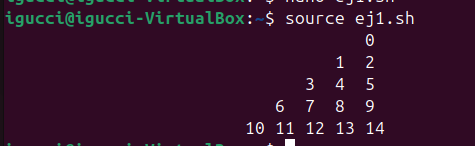
\includegraphics[width=0.5\linewidth]{Ej2piram.png}
    \caption{Ej2. Piramide}
\end{figure}
\newpage

\chapter{Consultas}
\section{Consulta 1}
Investigar la biografia de Dennis Ritchie, Linus Torvalds y Richard Stallman
\\
\vspace{5pt}
\subsection{{\bfseries Biografía Dennis Ritchie}} 

\vspace{5pt}
Dennis MacAlistair Ritchie fue un científico computacional estadounidense. Nació en Bronxville, Nueva York, el 9 de septiembre de 1941. Es reconocido por dos grandes contribuciones al mundo de la informática. Encargado de la reación del lenguaje de programación C,  es un lenguaje de programación de propósito general ampliamente utilizado por su eficiencia y por ser la base de muchos otros lenguajes. Estuvo en la co-creación del sistema operativo Unix Junto con Ken Thompson. Además, Ritchie desarrolló el sistema operativo Unix, que se ha convertido en la base de numerosos sistemas operativos modernos, incluyendo Linux y macOS.

\vspace{5pt}
Estos logros convierten a Ritchie en un pionero fundamental de la informática moderna. Su trabajo en C y Unix ha tenido un impacto profundo en el desarrollo de software y hardware a nivel mundial.

Además de C y Unix, Ritchie también participó en el desarrollo de otros lenguajes de programación como B y contribuyó a la investigación en diversos campos de la informática.

Recibió numerosos premios y reconocimientos a lo largo de su carrera, incluyendo el Premio Turing, el máximo galardón en computación. Falleció en Berkeley Heights, Nueva Jersey, en 2011.



\begin{figure}[htb]
  \centering
  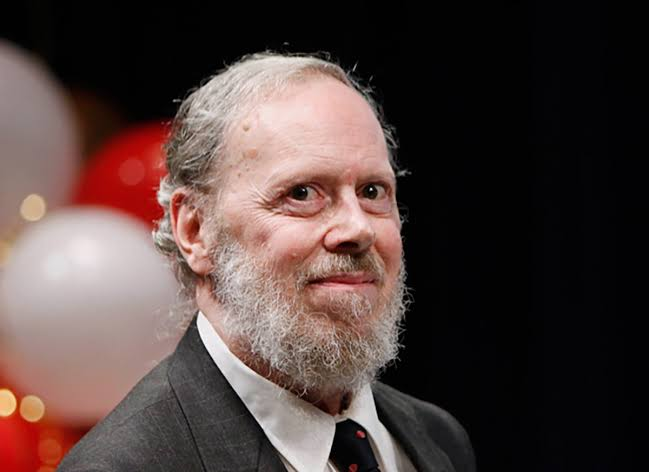
\includegraphics[width=0.3\linewidth, height=0.2\textheight]{D.R.png}
  \caption{Dennis Ritchie}
  \label{fig:etiqueta}
\end{figure}

\vspace{5pt}
\newpage
\subsection{{\bfseries Biografía Linus Torvalds}} 

\vspace{5pt}
Una de las personas que hizo una revolución tecnológica es Linus Torvalds, ya que todos los dispositivos electrónicos de alguna manera parten de Linux. Nacido el 28 de diciembre de 1969 en Hellsing,Finlandia. Desde muy pequeño, obtuvo su primer ordenador siendo el inicio de uno de los mejores informáticos que hayan existido, por esto en 1991, ya estando en la universidad, creó el sistema operativo Unix, después creó el Kernel Linux el cual sería fundamental para la creación de nuevos sistemas operativos en la actualidad.

\vspace{5pt}
Los sistemas operativos más utilizados como lo son Windows,IOS, Android entre otros, funcionan bajo el kernel de linux, es por esto que la creación de este kernel por parte de Linus Torvalds es muy importante, ya que al ser Open Source(código abierto), se pueden crear nuevos sistemas operativos que funcionen en cualquier dispositivo electrónico y al ser de código abierto, las personas con los conocimientos necesarios pueden aportar y mejorar las aplicaciones que se creen con el kernel de linux. Por lo que con la creación de Linux aporte de Torvalds, tuvo un impacto significativo en la forma en que se utiliza y desarrolla el software.

\vspace{5pt}
Linus Torvalds siempre ha apoyado el código abierto sin costo alguno, es por esto que es muy querido en la comunidad informática considerándolo un héroe, esto porque la iniciativa de Torvalds siempre fue mejorar el mundo sin fines de lucro.

\begin{figure}[htb]
  \centering
  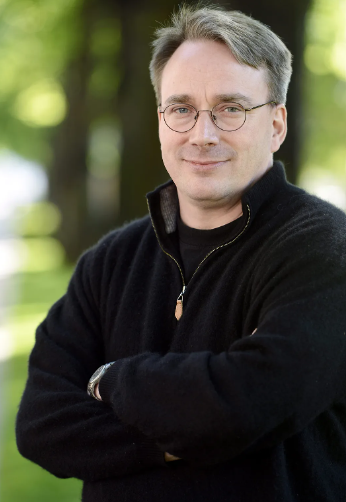
\includegraphics[width=0.2\linewidth, height=0.2\textheight]{L.T.png}
  \caption{Linus Torvalds}
  \label{fig:etiqueta}
\end{figure}
\vspace{5pt}

\subsection{{\bfseries Biografía Richard Stallman}} 
Richard Stallman es un programador y figura destacada del movimiento por el software libre. Nació el 16 de marzo de 1953 en Manhattan, Nueva York. Estudió física en la Universidad de Harvard y luego trabajó como hacker en el laboratorio de inteligencia artificial del MIT.

\vspace{5pt}
En la década de 1980, Stallman se vio frustrado por la comercialización en la industria del software y decidió crear una alternativa al software privativo. En 1983, inició el proyecto GNU con el objetivo de desarrollar un sistema operativo completamente libre. Fundó la organización sin ánimo de lucro Free Software Foundation para apoyar este proyecto. En 1991, el núcleo Linux fue lanzado bajo los términos de la GPL, lo que completó el sistema GNU.

\vspace{5pt}
Stallman también ha contribuido a la creación de GNUPedia, una enciclopedia de carácter libre considerada como precursora de Wikipedia. Además de sus logros informáticos, Stallman ha dado numerosas conferencias internacionales para difundir sus valores y promover el conocimiento libre.

\vspace{5pt}
Ha expresado su postura en contra de las patentes de software y ha participado activamente en el debate sobre este tema. Ha sido reconocido con varios premios por sus contribuciones al software libre.

\vspace{5pt}
Richard Stallman es una figura influyente en el movimiento por el software libre, conocido por su labor como programador, fundador del proyecto GNU y defensor de la libertad del software.

\begin{figure}[htb]
  \centering
  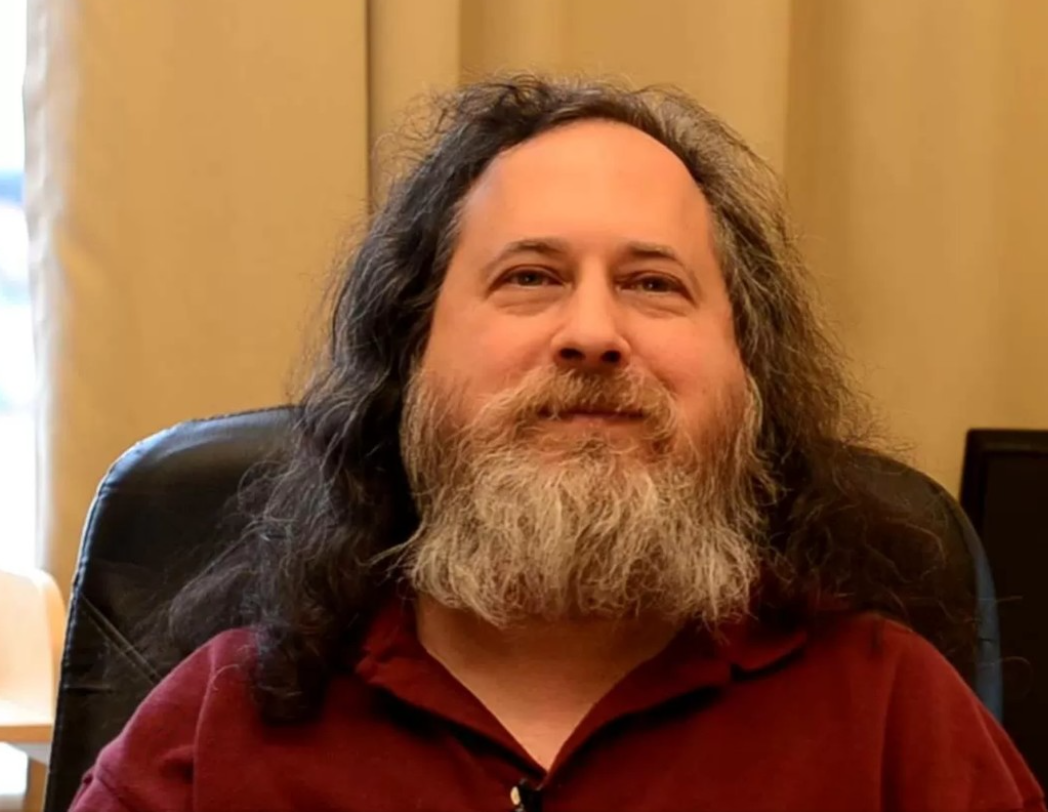
\includegraphics[width=0.3\linewidth]{R.S.1.png}
  \caption{Richard Stallman}
  \label{fig:etiqueta}
\end{figure}
\vspace{5pt}
\newpage

\section{Consulta 2}
\subsection{Arquitectura Android}
Android es un sistema operativo móvil desarrollado por Google. Desde su lanzamiento en 2008, se ha convertido en uno de los sistemas operativos móviles más populares del mundo, con una gran cantidad de dispositivos que ejecutan Android en todo el mundo.
La arquitectura de Android se basa en un sistema operativo Linux y está compuesta por varias capas y componentes que trabajan juntos para proporcionar la funcionalidad del sistema. Estas capas incluyen la capa de aplicaciones, la capa de marco de trabajo, la capa de bibliotecas y la capa de kernel. La capa de aplicaciones alberga las aplicaciones instaladas, mientras que el kernel se encarga de administrar los recursos del hardware.

\subsection{Arquitectura IOS}
La arquitectura de iOS se compone de cuatro capas principales: Cocoa Touch Layer, Media Layer, Core Services Layer, Core OS Layer y Kernel and Device Drivers. Estas capas trabajan juntas para proporcionar un entorno operativo completo y eficiente, permitiendo a los desarrolladores crear aplicaciones de alta calidad para dispositivos Apple. La integración estrecha entre hardware y software es una característica distintiva de la arquitectura de iOS, lo que contribuye a la experiencia de usuario ya que su interfaz grafica es intuitiva, al igual que la seguridad de servicio de almacenamiento que proporciona. 

\subsection{Arquitectura MacOs}
El sistema operativo macOS está basado en el kernel de Darwin, que a su vez se basa en UNIX. Esto ha sido una gran ventaja para muchos desarrolladores que aprecian la estabilidad y confiabilidad de UNIX, el sistema operativo macOS es mucho más complejo en su totalidad. Darwin es la base del sistema operativo macOS actual. Aunque Darwin es de código abierto, la última versión es macOs Ventura la cual se lanzó al público en octubre de 2022. Es importante destacar que Darwin es un sistema operativo sin interfaz gráfica de usuario.

\vspace{5pt}

\newpage
\chapter{Tareas}

\section{Tarea 1}
\subsection{10 Programas que automaticen procesos}
Realizar 10 ejercicios
\subsection{Ejercicio 1}
\begin{lstlisting}
#!/bin/bash
# Program Ejercicio 1
# Authors: Gustavo Aguas y Sebastian Paucar
# Explicacion del programa: Este programa suma los números del 1 al 100 utilizando un ciclo for.

sum=0
for i in {1..100}
do
  sum=$((sum + i))
done
echo "La suma de los números del 1 al 100 es: $sum"
# I love Linux
\end{lstlisting}
\begin{figure}[h]
    \centering
    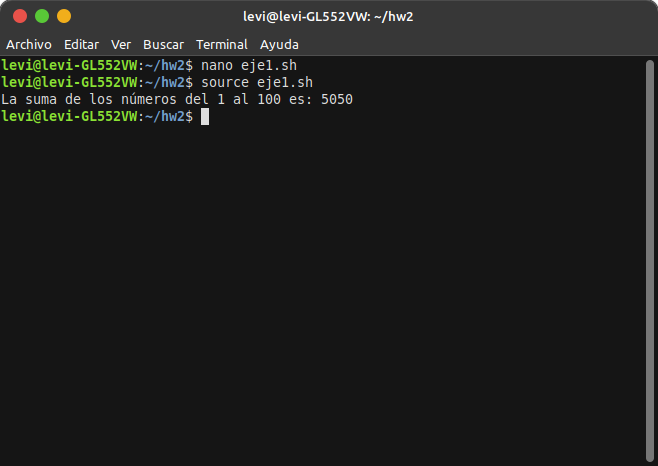
\includegraphics[width=0.8\linewidth]{Tarea2/teje1.png}
    \caption{ compilación del ejercicio 1}
\end{figure}

\newpage
\subsection{Ejercicio 2}
\begin{lstlisting}
#!/bin/bash
# Program Ejercicio 2
# Authors: Gustavo Aguas y Sebastian Paucar
# Explicacion del programa: Este programa cuenta del 1 al 10 utilizando un ciclo while.

count=1

while [ $count -le 10 ]
do
  echo "Número: $count"
  count=$((count + 1))
done
# I love Linux
\end{lstlisting}
\begin{figure}[h]
    \centering
    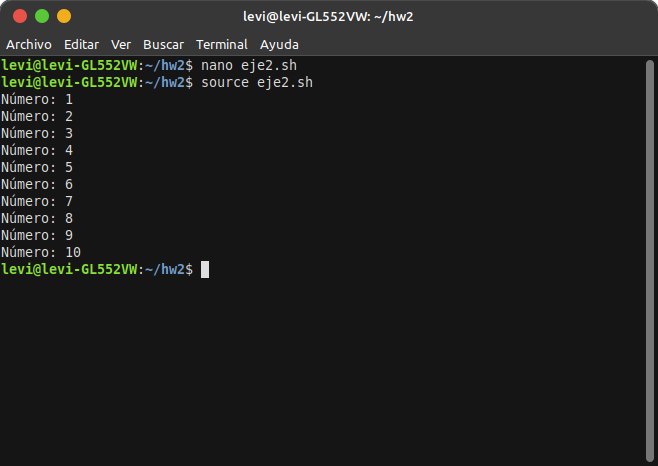
\includegraphics[width=0.8\linewidth]{Tarea2/teje2.png}
    \caption{ compilación del ejercicio 2}
\end{figure}
\newpage
\subsection{Ejercicio 3}
\begin{lstlisting}
#!/bin/bash
# Program Ejercicio 3
# Authors: Gustavo Aguas y Sebastian Paucar
# Explicacion del programa: Este programa verifica si un número ingresado es par o impar.

read -p "Ingresa un número: " num

if [ $((num % 2)) -eq 0 ]; then
  echo "El número $num es par."
else
  echo "El número $num es impar."
fi
#I love linux
\end{lstlisting}
\begin{figure}[h]
    \centering
    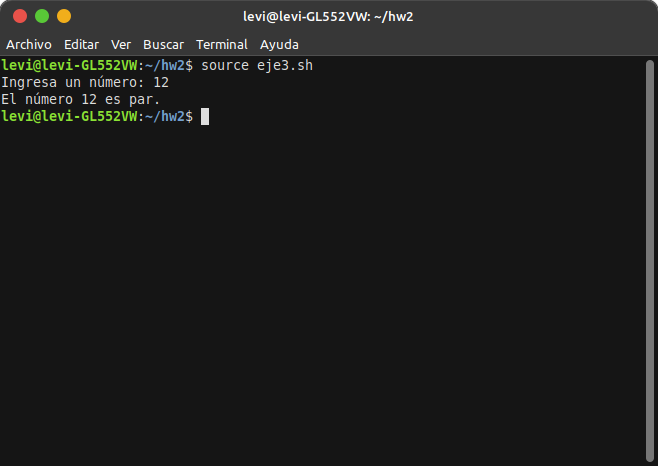
\includegraphics[width=0.8\linewidth]{Tarea2/teje32.png}
    \caption{ compilación del ejercicio 3}
\end{figure}
\newpage
\subsection{Ejercicio 4}
\begin{lstlisting}
#!/bin/bash
# Program Ejercicio 4
# Authors: Gustavo Aguas y Sebastian Paucar
# Explicacion del programa: Este programa muestra los nombres de los días de la semana utilizando un arreglo.

dias=("Lunes" "Martes" "Miércoles" "Jueves" "Viernes" "Sábado" "Domingo")

for dia in "${dias[@]}"
do
  echo "Día: $dia"
done
#I love linux
\end{lstlisting}
\begin{figure}[h]
    \centering
    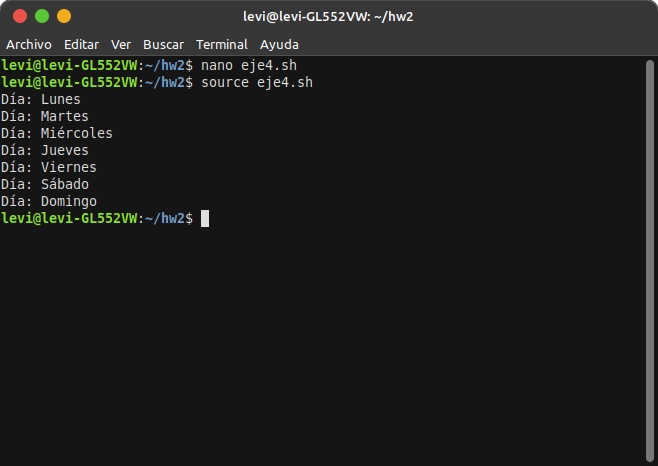
\includegraphics[width=0.8\linewidth]{Tarea2/teje4.png}
    \caption{ compilación del ejercicio 4}
\end{figure}
\newpage
\subsection{Ejercicio 5}
\begin{lstlisting}
#!/bin/bash
# Program Ejercicio 5
# Authors: Gustavo Aguas y Sebastian Paucar
# Explicacion del programa: Este programa imprime la tabla de multiplicar del número ingresado.

read -p "Ingresa un número: " num

for i in {1..10}
do
  echo "$num x $i = $((num * i))"
done
#I love linux
\end{lstlisting}
\begin{figure}[h]
    \centering
    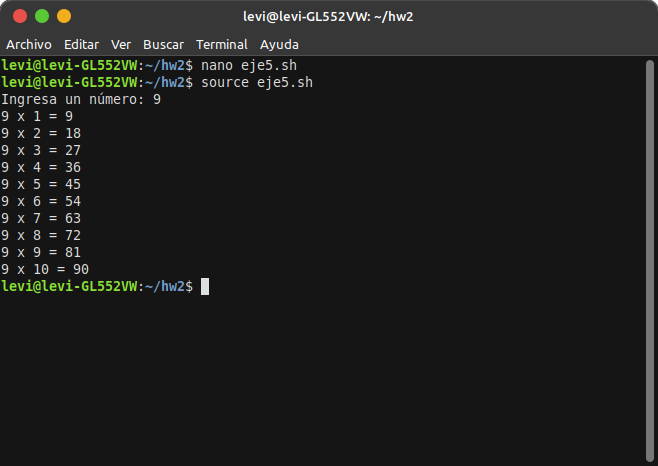
\includegraphics[width=0.8\linewidth]{Tarea2/teje5.png}
    \caption{ compilación del ejercicio 5}
\end{figure}
\newpage
\subsection{Ejercicio 6}

\begin{lstlisting}
#!/bin/bash
# Program Ejercicio 6
# Authors: Gustavo Aguas y Sebastian Paucar
# Explicacion del programa: Este programa encuentra el número más grande en un arreglo.

numeros=(23 45 67 89 12 34 56)

max=${numeros[0]}

for num in "${numeros[@]}"
do
  if [ $num -gt $max ]; then
    max=$num
  fi
done

echo "El número más grande es: $max"
#I love linux
\end{lstlisting}
\begin{figure}[h]
    \centering
    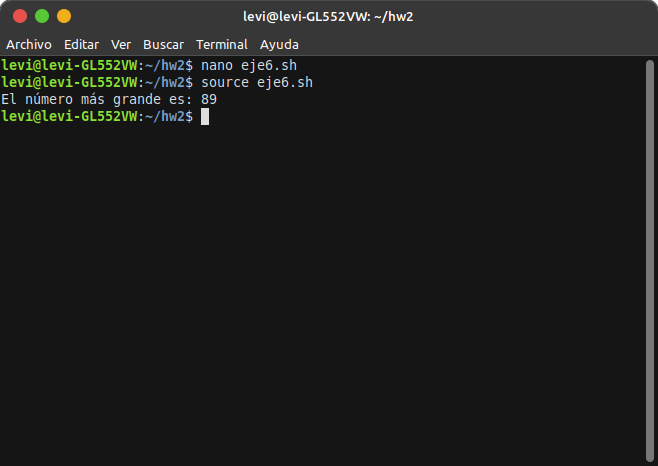
\includegraphics[width=0.8\linewidth]{Tarea2/teje6.png}
    \caption{ compilación del ejercicio 6}
\end{figure}
\newpage
\subsection{Ejercicio 7}
\begin{lstlisting}
#!/bin/bash
# Program Ejercicio 7
# Authors: Gustavo Aguas y Sebastian Paucar
# Explicacion del programa: Este programa cuenta el número de vocales en una cadena ingresada.

read -p "Ingresa una cadena: " cadena

vocales=0

for (( i=0; i<${#cadena}; i++ ))
do
  char=${cadena:$i:1}
  if [[ "$char" =~ [aeiouAEIOU] ]]; then
    vocales=$((vocales + 1))
  fi
done

echo "La cadena contiene $vocales vocales."
#I love linux
\end{lstlisting}
\begin{figure}[h]
    \centering
    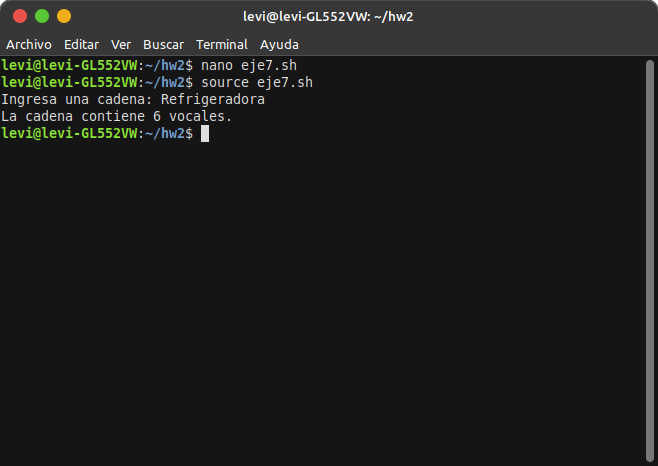
\includegraphics[width=0.8\linewidth]{Tarea2/teje7.png}
    \caption{ compilación del ejercicio 7}
\end{figure}
\newpage
\subsection{Ejercicio 8}
\begin{lstlisting}
#!/bin/bash
# Program Ejercicio 8
# Authors: Gustavo Aguas y Sebastian Paucar
# Explicacion del programa: Este programa verifica si un número ingresado es primo.

read -p "Ingresa un número: " num
es_primo=1

if [ $num -le 1 ]; then
  es_primo=0
else
  for ((i=2; i<=num/2; i++))
  do
    if [ $((num % i)) -eq 0 ]; then
      es_primo=0
      break
    fi
  done
fi

if [ $es_primo -eq 1 ]; then
  echo "El número $num es primo."
else
  echo "El número $num no es primo."
fi
#I love linux
\end{lstlisting}
\begin{figure}[h]
    \centering
    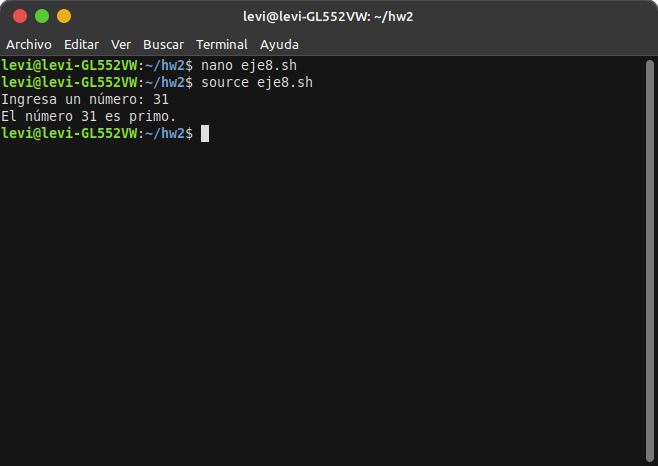
\includegraphics[width=0.6\linewidth]{Tarea2/teje8.png}
    \caption{ compilación del ejercicio 8}
\end{figure}
\newpage
\subsection{Ejercicio 9}
\begin{lstlisting}
#!/bin/bash
# Program Ejercicio 9
# Authors: Gustavo Aguas y Sebastian Paucar
# Explicacion del programa: Este programa invierte una cadena ingresada.

read -p "Ingresa una cadena: " cadena

longitud=${#cadena}

for (( i=$longitud-1; i>=0; i-- ))
do
  invertida="$invertida${cadena:$i:1}"
done

echo "La cadena invertida es: $invertida"
#I love linux
\end{lstlisting}
\begin{figure}[h]
    \centering
    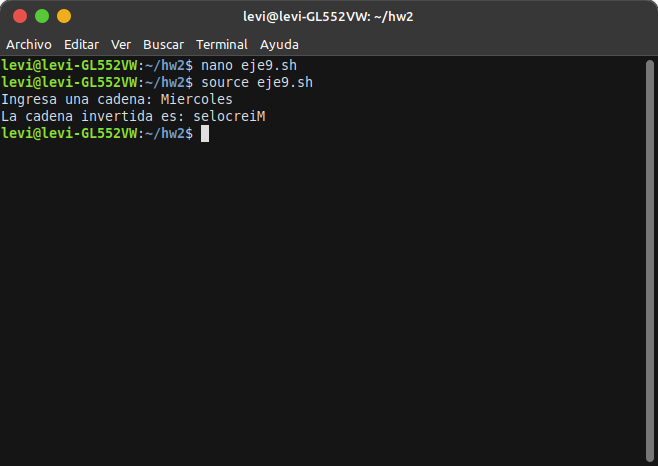
\includegraphics[width=0.8\linewidth]{Tarea2/teje9.png}
    \caption{ compilación del ejercicio 9}
\end{figure}
\newpage
\subsection{Ejercicio 10}

\begin{lstlisting}
#!/bin/bash
# Program Ejercicio 10
# Authors: Gustavo Aguas y Sebastian Paucar
# Explicacion del programa: Este programa calcula el factorial de un número ingresado.

read -p "Ingresa un número: " num
factorial=1

for (( i=1; i<=num; i++ ))
do
  factorial=$((factorial * i))
done

echo "El factorial de $num es: $factorial"
\end{lstlisting}
\begin{figure}[h]
    \centering
    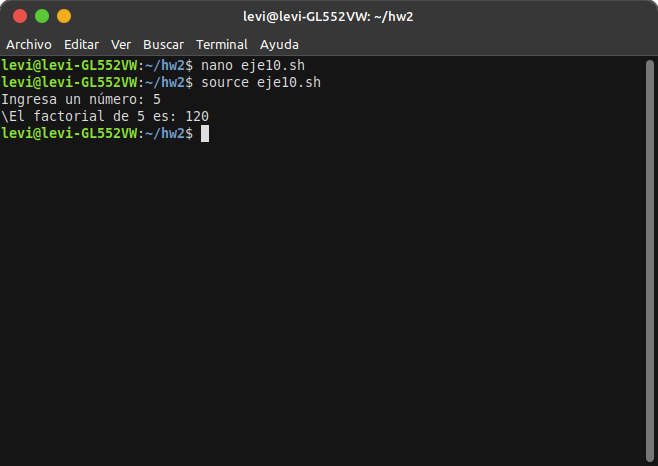
\includegraphics[width=0.8\linewidth]{Tarea2/teje10.png}
    \caption{ compilación del ejercicio 10}
\end{figure}

\newpage
\section{Tarea 2}

\subsection{Ejercicios de programación en Shell con while, if}

Realizar 15 ejercicios

\subsection{Ejercicio 1}

El menor de dos numeros
\begin{lstlisting}
#!/bin/bash
#Program Ejercicio 1
#Authors: Gustavo Aguas y Sebastian Paucar
#Date: 29-05-2023
clear
echo "Ingrese el 1er numero";
read num1;
echo "Ingrese el 2do numero";
read num2;
if [ $num1 -lt $num2 ]; then
echo "el menor  numero es: $num1"
elif [ $num2 -lt $num1 ]; then
echo "El menor es: $num2";
else 
echo "$num1, $num2 son iguales";
fi
#I love linux

\end{lstlisting}
\begin{figure}[h]
    \centering
    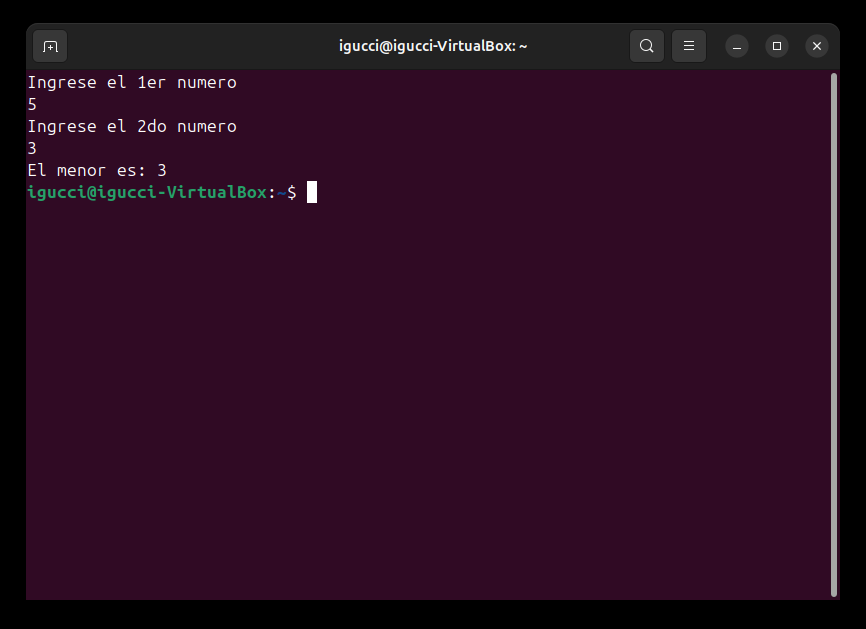
\includegraphics[width=0.5\linewidth]{Ej1.png}
    \caption{Ejercicio 1}
 
\end{figure}


\newpage
\subsection{Ejercicio 2}

Operaciones basicas
\begin{lstlisting}
#!/bin/bash
#Program Ejercicio 2
#Authors: Gustavo Aguas y Sebastian Paucar
#Date: 29-05-2023
echo "Ingrese el primer número entero positivo:"
read num1

echo "Ingrese el segundo número entero positivo:"
read num2

suma=$(expr $num1 + $num2)
resta=$(expr $num1 - $num2)
multiplicacion=$(expr $num1 \* $num2)
division=$(expr $num1 / $num2)

echo "Resultados:"
echo "Suma: $num1 + $num2 = $suma"
echo "Resta: $num1 - $num2 = $resta"
echo "Multiplicación: $num1 * $num2 = $multiplicacion"
echo "División: $num1 / $num2 = $division"

\end{lstlisting}
\begin{figure}[h]
    \centering
    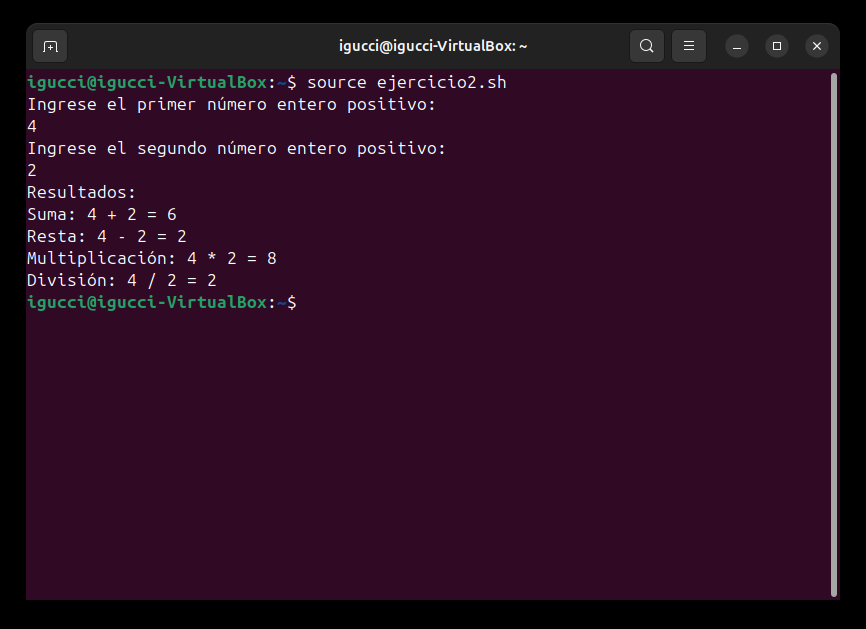
\includegraphics[width=0.5\linewidth]{Ej2.png}
    \caption{Ejercicio 2}

\end{figure}

\newpage
\subsection{Ejercicio 3}

Secuencia hasta el 10
\begin{lstlisting}
#!/bin/bash
#Program Ejercicio 3
#Authors: Gustavo Aguas y Sebastian Paucar
#Date: 29-05-2023
cont=0
while [ $cont -lt 11 ]
do
echo $cont
cont=$((cont + 1))
done
# I LOVE LINUX
\end{lstlisting}
\begin{figure}[h]
    \centering
    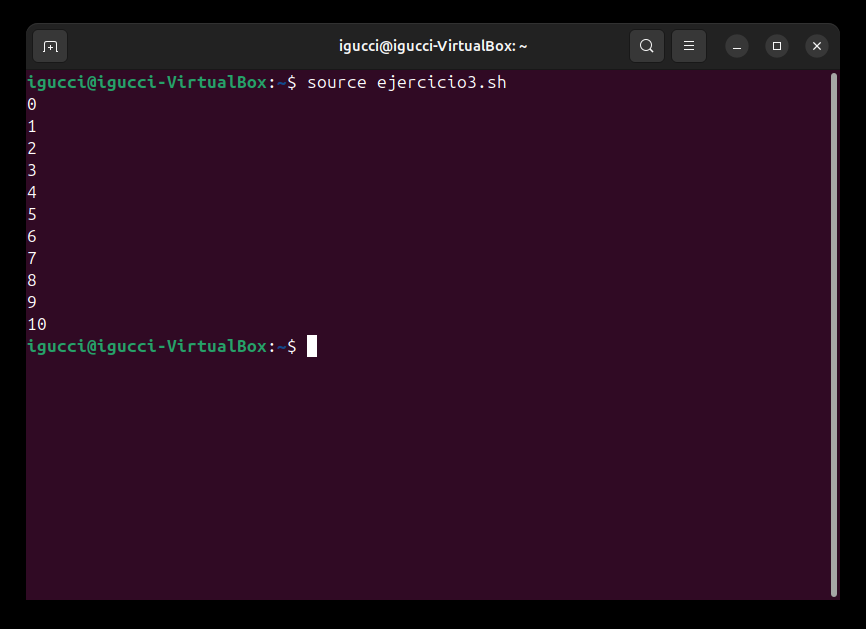
\includegraphics[width=0.5\linewidth]{Ej3.png}
    \caption{Ejercicio 3}

\end{figure}

\newpage
\subsection{Ejercicio 4}

Primeros 20 multiplos de 3
\begin{lstlisting}
#!/bin/bash
#Program Ejercicio 4
#Authors: Gustavo Aguas y Sebastian Paucar
#Date: 29-05-2023
# Imprimir los primeros 20 múltiplos de 3
echo "Los primeros 20 múltiplos de 3 son:"
for (( i=1; i<=20; i++ )); do
  multiplo=$((i * 3))
  echo $multiplo
done

\end{lstlisting}
\begin{figure}[h]
    \centering
    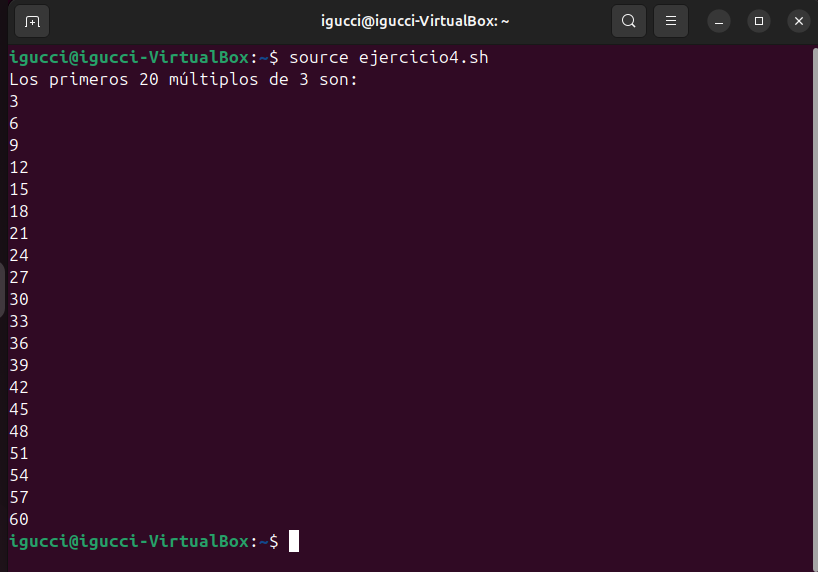
\includegraphics[width=0.5\linewidth]{Ej4.png}
    \caption{Ejercicio 4}

\end{figure}

\newpage
\subsection{Ejercicio 5}

Tabla de multiplicar del num 4 hasta el  20
\begin{lstlisting}
#!/bin/bash
#Program Ejercicio 5
#Authors: Gustavo Aguas y Sebastian Paucar
#Date: 29-05-2023
# Leer un número entero positivo
echo "Ingrese un número entero positivo:"
read num

# Calcular y mostrar la tabla de multiplicar hasta el 20
for ((i = 1; i <= 20; i++)); do
  resultado=$((num * i))
  echo "$num x $i = $resultado"
done

\end{lstlisting}
\begin{figure}[h]
    \centering
    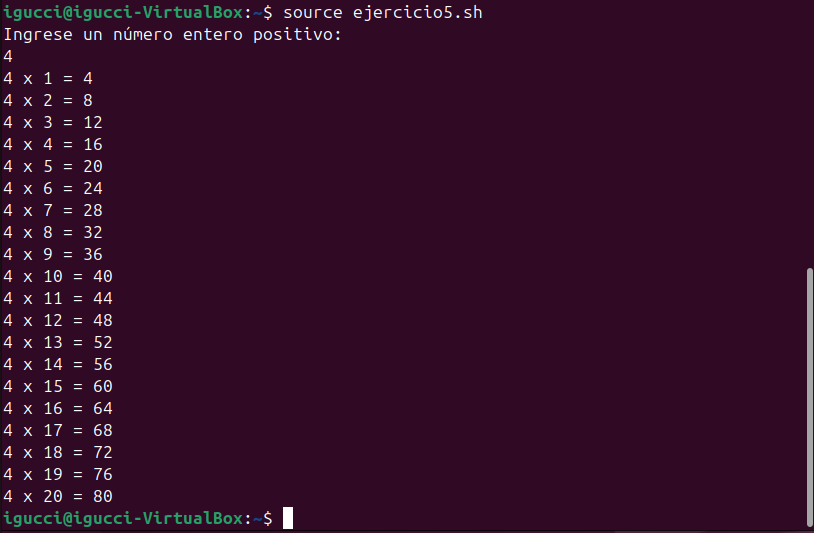
\includegraphics[width=0.5\linewidth]{Ej5.png}
    \caption{Ejercicio 5}

\end{figure}
\newpage
\subsection{Ejercicio 6}
Verificar si un número es positivo, negativo o cero

\begin{lstlisting}
#!/bin/bash
#Program Ejercicio 6
#Authors: Gustavo Aguas y Sebastian Paucar
#Date: 29-05-2023
echo "Ingrese un número:"
read num

if (( num > 0 )); then
  echo "$num es positivo"
elif (( num < 0 )); then
  echo "$num es negativo"
else
  echo "$num es cero"
fi

echo "I love Linux"


\end{lstlisting}
\begin{figure}[h]
    \centering
    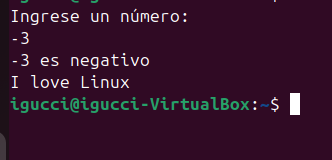
\includegraphics[width=0.5\linewidth]{image.png}
    \caption{Ejercicio 6}
\end{figure}
\newpage
\subsection{Ejercicio 7}

Imprimir los primeros 10 números pares y su suma 
\begin{lstlisting}
#!/bin/bash
#Program Ejercicio 7
#Authors: Gustavo Aguas y Sebastian Paucar
#Date: 29-05-2023
suma=0
for (( i = 1; i <= 10; i++ )); do
  num=$(( i * 2 ))
  echo "Número par: $num"
  suma=$(( suma + num ))
done

echo "La suma de los primeros 10 números pares es $suma"

echo "I love Linux"

\end{lstlisting}
\begin{figure}[h]
    \centering
    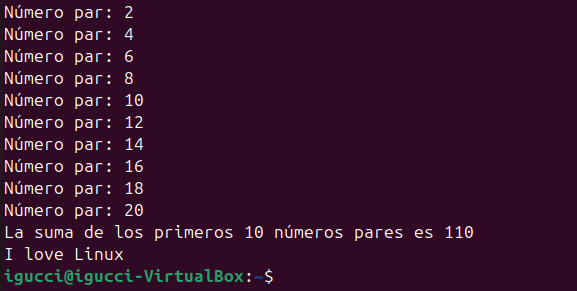
\includegraphics[width=0.5\linewidth]{Ej7.png}
    \caption{Ejercicio 7}
\end{figure}
\newpage
\subsection{Ejercicio 8}

Contar del 1 al 20 y mostrar si cada número es par o impar
\begin{lstlisting}
#!/bin/bash
#Program Ejercicio 8
#Authors: Gustavo Aguas y Sebastian Paucar
#Date: 29-05-2023
for (( i = 1; i <= 20; i++ )); do
  if (( i % 2 == 0 )); then
    echo "$i es par"
  else
    echo "$i es impar"
  fi
done

echo "I love Linux"

\end{lstlisting}
\begin{figure}[h]
    \centering
    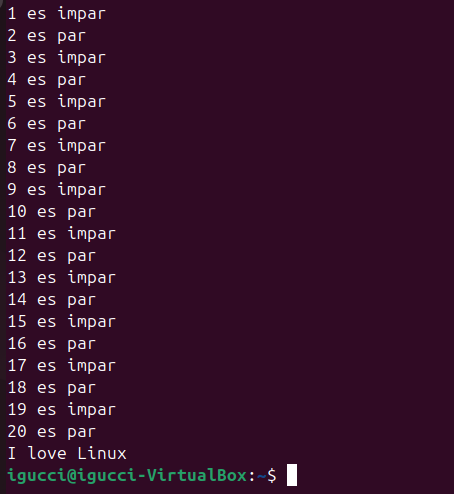
\includegraphics[width=0.5\linewidth]{Ej8.png}
    \caption{Ejercicio 8}
\end{figure}
\newpage
\subsection{Ejercicio 9}
 Calcular la suma de los números del 1 al 100 y mostrar el resultado
\begin{lstlisting}
#!/bin/bash
#Program Ejercicio 9
#Authors: Gustavo Aguas y Sebastian Paucar
#Date: 29-05-2023
suma=0
for (( i = 1; i <= 100; i++ )); do
  suma=$(( suma + i ))
done

echo "La suma de los números del 1 al 100 es $suma"

echo "I love Linux"

\end{lstlisting}

\begin{figure}[h]
    \centering
    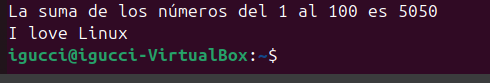
\includegraphics[width=0.5\linewidth]{Ej9.png}
    \caption{Ejercicio 9}
\end{figure}
\newpage
\subsection{Ejercicio 10}
Imprimir la tabla de multiplicar de un número hasta el 20

\begin{lstlisting}
#!/bin/bash
#Program Ejercicio 10
#Authors: Gustavo Aguas y Sebastian Paucar
#Date: 29-05-2023
echo "Ingrese un número entero positivo:"
read num

for (( i = 1; i <= 20; i++ )); do
  resultado=$(( num * i ))
  echo "$num x $i = $resultado"
done

echo "I love Linux"

\end{lstlisting}

\begin{figure}[h]
    \centering
    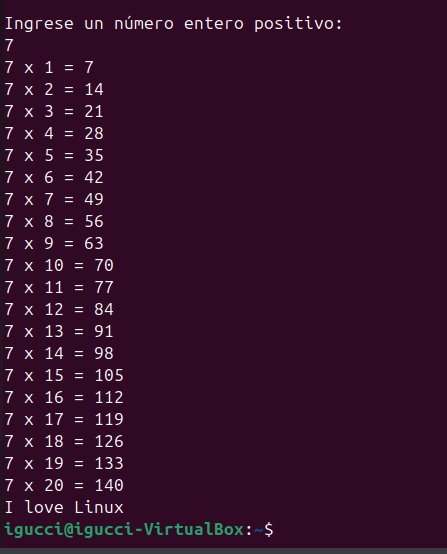
\includegraphics[width=0.5\linewidth]{Ej10.png}
    \caption{Ejercicio 10}
\end{figure}
\newpage
\subsection{Ejercicio 11}
Contar las letras de una cadena y mostrar cuántas son vocales y cuántas son consonantes

\begin{lstlisting}
#!/bin/bash
#Program Ejercicio 11
#Authors: Gustavo Aguas y Sebastian Paucar
#Date: 29-05-2023
echo "Ingrese una cadena de texto:"
read cadena

longitud=${#cadena}
vocales=0
consonantes=0

for (( i = 0; i < longitud; i++ )); do
  letra=${cadena:$i:1}
  if [[ $letra =~ [aeiouAEIOU] ]]; then
    vocales=$(( vocales + 1 ))
  elif [[ $letra =~ [bcdfghjklmnpqrstvwxyzBCDFGHJKLMNPQRSTVWXYZ] ]]; then
    consonantes=$(( consonantes + 1 ))
  fi
done

echo "La cadena tiene $longitud caracteres, de los cuales $vocales son vocales y $consonantes son consonantes."

echo "I love Linux"


\end{lstlisting}
\begin{figure}[h]
    \centering
    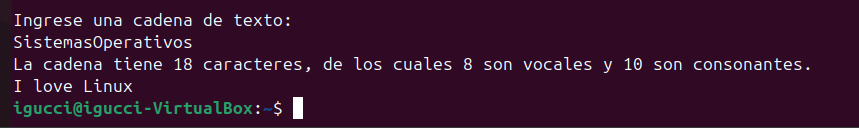
\includegraphics[width=1\linewidth]{Ej11.png}
    \caption{Ejercicio 11}
\end{figure}
\newpage
\subsection{Ejercicio 12}

Comprobar si un número es múltiplo de 3 o 5 y mostrar todos los múltiplos de 3 o 5 hasta 50

\begin{lstlisting}
#!/bin/bash
#Program Ejercicio 12
#Authors: Gustavo Aguas y Sebastian Paucar
#Date: 29-05-2023
echo "Ingrese un número:"
read num

if (( num % 3 == 0 )); then
  echo "$num es múltiplo de 3"
elif (( num % 5 == 0 )); then
  echo "$num es múltiplo de 5"
else
  echo "$num no es múltiplo de 3 ni de 5"
fi

echo "Múltiplos de 3 o 5 hasta 50:"
for (( i = 1; i <= 50; i++ )); do
  if (( i % 3 == 0 || i % 5 == 0 )); then
    echo $i
  fi
done

echo "I love Linux"

\end{lstlisting}
\begin{figure}[h]
    \centering
    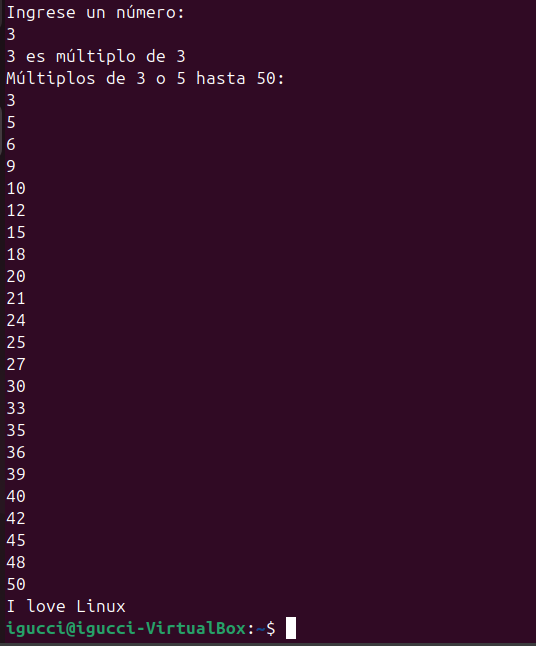
\includegraphics[width=0.5\linewidth]{Ej12.png}
    \caption{Ejercicio 12}
\end{figure}
\newpage
\subsection{Ejercicio 13}
Sumar los primeros N números pares
\begin{lstlisting}
#!/bin/bash
#Program Ejercicio 13
#Authors: Gustavo Aguas y Sebastian Paucar
#Date: 29-05-2023
echo "Ingrese un número entero positivo N:"
read N

suma=0
for (( i = 1; i <= N; i++ )); do
  num=$(( i * 2 ))
  suma=$(( suma + num ))
done

echo "La suma de los primeros $N números pares es $suma"

echo "I love Linux"

\end{lstlisting}
\begin{figure}[h]
    \centering
    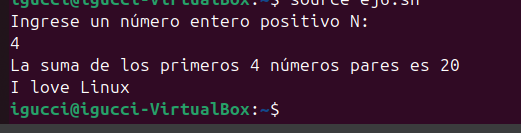
\includegraphics[width=1\linewidth]{Ej13.png}
    \caption{Ejercicio 13}
\end{figure}
\newpage
\subsection{Ejercicio 14}
Imprimir los números primos del 1 al 50
\begin{lstlisting}
#!/bin/bash
#Program Ejercicio 14
#Authors: Gustavo Aguas y Sebastian Paucar
#Date: 29-05-2023
echo "Números primos del 1 al 50:"
for (( num = 2; num <= 50; num++ )); do
  es_primo=1
  for (( i = 2; i <= num / 2; i++ )); do
    if (( num % i == 0 )); then
      es_primo=0
      break
    fi
  done
  if (( es_primo == 1 )); then
    echo $num
  fi
done

echo "I love Linux"

\end{lstlisting}
\begin{figure}[h]
    \centering
    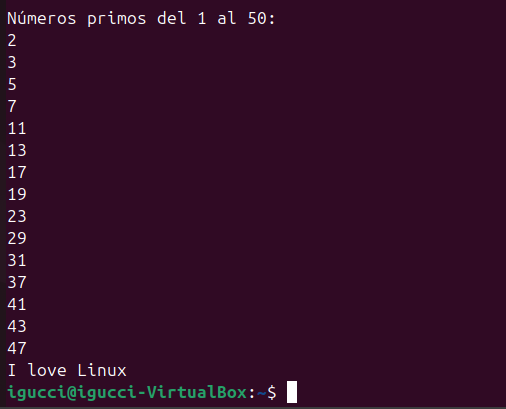
\includegraphics[width=0.5\linewidth]{Ej14.png}
    \caption{Ejercicio 14}
\end{figure}
\newpage
\subsection{Ejercicio 15}
Verificar si una cadena es un palíndromo
\begin{lstlisting}
#!/bin/bash
#Program Ejercicio 15
#Authors: Gustavo Aguas y Sebastian Paucar
#Date: 29-05-2023
echo "Ingrese una cadena de texto:"
read cadena

cadena_invertida=$(echo $cadena | rev)

if [ "$cadena" == "$cadena_invertida" ]; then
  echo "La cadena es un palíndromo"
else
  echo "La cadena no es un palíndromo"
fi

echo "I love Linux"

\end{lstlisting}
\begin{figure}[h]
    \centering
    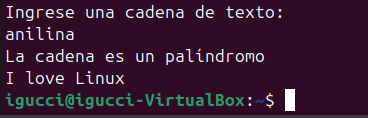
\includegraphics[width=0.5\linewidth]{Ej15.png}
    \caption{Ejercicio 15}
\end{figure}
\newpage
\section{Tarea 3}
\subsection{Ejercicios de series}
Realizar 10 ejercicios
\subsection{Ejercicio 1}
\begin{lstlisting}
#!/bin/bash
# Program Ejercicio 1
# Authors: Gustavo Aguas y Sebastian Paucar
# Explicacion del programa: Serie de números del 1 al 20 y su suma total
sum=0
for i in {1..20}; do
    echo $i
    sum=$((sum + i))
done
echo "La suma total es: $sum"
# I love Linux
\end{lstlisting}
\begin{figure}
    \centering
    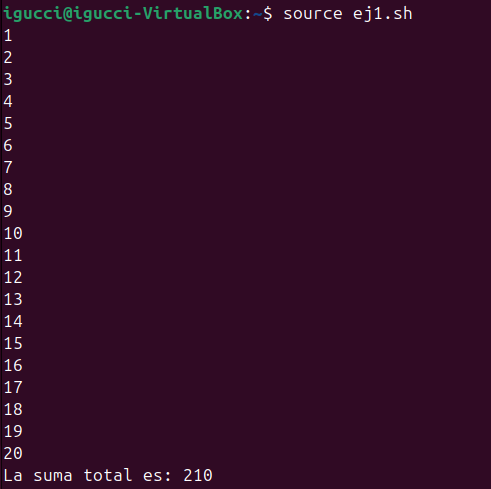
\includegraphics[width=0.8\linewidth]{series/ej1.png}
    \caption{Ejercicio 1}
\end{figure}

\newpage
\subsection{Ejercicio 2}
\begin{lstlisting}
#!/bin/bash
# Program Ejercicio 2
# Authors: Gustavo Aguas y Sebastian Paucar
# Explicacion del programa: Serie de números pares del 2 al 40 y su promedio
sum=0
count=0
for i in {2..40..2}; do
    echo $i
    sum=$((sum + i))
    count=$((count + 1))
done
average=$(echo "scale=2; $sum / $count" | bc)
echo "El promedio es: $average"
# I love Linux
\end{lstlisting}
\begin{figure}
    \centering
    \includegraphics[width=0.75\linewidth]{series/ej2.png}
    \caption{Ejercicio 2}
\end{figure}
\newpage
\subsection{Ejercicio 3}
\begin{lstlisting}
#!/bin/bash
# Program Ejercicio 3
# Authors: Gustavo Aguas y Sebastian Paucar
# Explicacion del programa: Serie de números impares del 1 al 39 y su producto total

product=1
for i in {1..39..2}; do
    echo $i
    product=$((product * i))
done
echo "El producto total es: $product"
#I love linux
\end{lstlisting}
\begin{figure}
    \centering
    \includegraphics[width=0.75\linewidth]{series/ej3.png}
    \caption{Ejercicio 3}
\end{figure}
\newpage
\subsection{Ejercicio 4}
\begin{lstlisting}
#!/bin/bash
# Program Ejercicio 4
# Authors: Gustavo Aguas y Sebastian Paucar
# Explicacion del programa: Serie de múltiplos de 3 hasta 60 y contar cuántos hay

count=0
for ((i=3; i<=60; i+=3)); do
    echo $i
    count=$((count + 1))
done
echo "El número de múltiplos de 3 es: $count"
#I love linux
\end{lstlisting}
\begin{figure}
    \centering
    \includegraphics[width=0.75\linewidth]{series/ej4.png}
    \caption{Ejercicio 4}
\end{figure}
\newpage
\subsection{Ejercicio 5}
\begin{lstlisting}
#!/bin/bash
# Program Ejercicio 5
# Authors: Gustavo Aguas y Sebastian Paucar
# Explicacion del programa: Serie de Fibonacci (los primeros 15 números) y su suma

a=0
b=1
sum=$a
echo $a
echo $b
for ((i=2; i<15; i++)); do
    c=$((a + b))
    echo $c
    sum=$((sum + c))
    a=$b
    b=$c
done
echo "La suma de la serie Fibonacci es: $sum"
#I love linux
\end{lstlisting}
\begin{figure}
    \centering
    \includegraphics[width=0.75\linewidth]{series/ej5.png}
    \caption{Ejercicio 5}
\end{figure}
\newpage
\subsection{Ejercicio 6}

\begin{lstlisting}
#!/bin/bash
# Program Ejercicio 6
# Authors: Gustavo Aguas y Sebastian Paucar
# Explicacion del programa: Serie de cuadrados de los números del 1 al 15 y su suma

sum=0
for i in {1..15}; do
    square=$(echo "$i^2" | bc)
    echo "$i^2 = $square"
    sum=$(echo "$sum + $square" | bc)
done
echo "La suma de los cuadrados es: $sum"
#I love linux
\end{lstlisting}
\begin{figure}
    \centering
    \includegraphics[width=0.75\linewidth]{series/ej6.png}
    \caption{Ejercicio 6}
\end{figure}
\newpage
\subsection{Ejercicio 7}
\begin{lstlisting}
#!/bin/bash
# Program Ejercicio 7
# Authors: Gustavo Aguas y Sebastian Paucar
# Explicacion del programa: Serie de cubos de los números del 1 al 10 y su promedio

sum=0
count=0
for i in {1..10}; do
    cube=$(echo "$i^3" | bc)
    echo "$i^3 = $cube"
    sum=$(echo "$sum + $cube" | bc)
    count=$((count + 1))
done
average=$(echo "scale=2; $sum / $count" | bc)
echo "El promedio de los cubos es: $average"
#I love linux
\end{lstlisting}
\begin{figure}
    \centering
    \includegraphics[width=0.75\linewidth]{series/ej7.png}
    \caption{Ejercicio 7}
\end{figure}
\newpage
\subsection{Ejercicio 8}
\begin{lstlisting}
#!/bin/bash
# Program Ejercicio 8
# Authors: Gustavo Aguas y Sebastian Paucar
# Explicacion del programa: Serie de los primeros 10 números con dos decimales y su suma

sum=0
for i in {1..10}; do
    value=$(echo "scale=2; $i/1" | bc)
    echo $value
    sum=$(echo "$sum + $value" | bc)
done
echo "La suma total es: $sum"
#I love linux
\end{lstlisting}
\begin{figure}
    \centering
    \includegraphics[width=0.75\linewidth]{series/ej8.png}
    \caption{Ejercicio 8}
\end{figure}
\newpage
\subsection{Ejercicio 9}
\begin{lstlisting}
#!/bin/bash
# Program Ejercicio 9
# Authors: Gustavo Aguas y Sebastian Paucar
# Explicacion del programa: Serie de los primeros 10 números factoriales y su suma

factorial() {
    if [ $1 -le 1 ]; then
        echo 1
    else
        echo "$1 * $(factorial $(($1 - 1)))" | bc
    fi
}

sum=0
for i in {1..10}; do
    fact=$(factorial $i)
    echo "$i! = $fact"
    sum=$(echo "$sum + $fact" | bc)
done
echo "La suma de los factoriales es: $sum"
#I love linux
\end{lstlisting}
\begin{figure}
    \centering
    \includegraphics[width=0.75\linewidth]{series/ej9.png}
    \caption{Ejercicio 9}
\end{figure}
\newpage
\subsection{Ejercicio 10}

\begin{lstlisting}
#!/bin/bash
# Program Ejercicio 10
# Authors: Gustavo Aguas y Sebastian Paucar
# Explicacion del programa: Serie de los primeros 10 números con raíz cuadrada y su suma

sum=0
for i in {1..10}; do
    sqrt=$(echo "scale=2; sqrt($i)" | bc)
    echo "sqrt($i) = $sqrt"
    sum=$(echo "$sum + $sqrt" | bc)
done
echo "La suma de las raíces cuadradas es: $sum"
#I love linux
\end{lstlisting}
\begin{figure}
    \centering
    \includegraphics[width=0.75\linewidth]{series/ej10.png}
    \caption{Ejercicio 10}
\end{figure}

\newpage
\section{Tarea 4}
\subsection{Permisos numericos}
Realizar 10 ejercicios
\subsection{Ejercicio 1}
\begin{lstlisting}
#!/bin/bash
# Program Ejercicio 1
# Authors: Gustavo Aguas y Sebastian Paucar
# Explicacion del programa: Crear un archivo file1.txt y otorgarle permisos de lectura, escritura y ejecución al usuario; solo lectura y ejecución al grupo y sin permisos a otros:

touch file1.txt
chmod 750 file1.txt
ls -l file1.txt
# I love Linux
\end{lstlisting}
\begin{figure}
    \centering
    \includegraphics[width=1\linewidth]{pnum/ej1.png}
    \caption{Ejercicio 1}
\end{figure}

\newpage
\subsection{Ejercicio 2}
\begin{lstlisting}
#!/bin/bash
# Program Ejercicio 2
# Authors: Gustavo Aguas y Sebastian Paucar
# Explicacion del programa: Crear un archivo file2.txt y otorgarle permisos de lectura y escritura al usuario; solo lectura al grupo y sin permisos a otros:

touch file2.txt
chmod 640 file2.txt
ls -l file2.txt
# I love Linux
\end{lstlisting}
\begin{figure}
    \centering
    \includegraphics[width=1\linewidth]{pnum/ej2.png}
    \caption{Ejercicio 2}
\end{figure}
\newpage
\subsection{Ejercicio 3}
\begin{lstlisting}
#!/bin/bash
# Program Ejercicio 3
# Authors: Gustavo Aguas y Sebastian Paucar
# Explicacion del programa: Crear un archivo file3.txt y otorgarle permisos de lectura y escritura al usuario; sin permisos al grupo y otros:

touch file3.txt
chmod 600 file3.txt
ls -l file3.txt
#I love linux
\end{lstlisting}
\begin{figure}
    \centering
    \includegraphics[width=1\linewidth]{pnum/ej3.png}
    \caption{Ejercicio 3}
\end{figure}
\newpage
\subsection{Ejercicio 4}
\begin{lstlisting}
#!/bin/bash
# Program Ejercicio 4
# Authors: Gustavo Aguas y Sebastian Paucar
# Explicacion del programa: Crear un archivo file4.txt y otorgarle permisos de lectura, escritura y ejecución al usuario y grupo; solo lectura y ejecución a otros:

touch file4.txt
chmod 775 file4.txt
ls -l file4.txt
#I love linux
\end{lstlisting}
\begin{figure}
    \centering
    \includegraphics[width=1\linewidth]{pnum/ej5.png}
    \caption{Ejercicio 4}
\end{figure}
\newpage
\subsection{Ejercicio 5}
\begin{lstlisting}
#!/bin/bash
# Program Ejercicio 5
# Authors: Gustavo Aguas y Sebastian Paucar
# Explicacion del programa: Crear un archivo file5.txt y otorgarle permisos de lectura y escritura al usuario y grupo; sin permisos a otros:

touch file5.txt
chmod 660 file5.txt
ls -l file5.txt
#I love linux
\end{lstlisting}
\begin{figure}
    \centering
    \includegraphics[width=1\linewidth]{pnum/ej5.png}
    \caption{Ejercicio 5}
\end{figure}
\newpage
\subsection{Ejercicio 6}

\begin{lstlisting}
#!/bin/bash
# Program Ejercicio 6
# Authors: Gustavo Aguas y Sebastian Paucar
# Explicacion del programa: Crear un archivo file6.txt y otorgarle permisos de solo lectura a todos:
bash

touch file6.txt
chmod 444 file6.txt
ls -l file6.txt
#I love linux
\end{lstlisting}
\begin{figure}
    \centering
    \includegraphics[width=1\linewidth]{pnum/ej6.png}
    \caption{Ejercicio 6}
\end{figure}
\newpage
\subsection{Ejercicio 7}
\begin{lstlisting}
#!/bin/bash
# Program Ejercicio 7
# Authors: Gustavo Aguas y Sebastian Paucar
# Explicacion del programa: Crear un archivo file7.txt y otorgarle permisos de escritura y ejecución al usuario; solo ejecución al grupo y otros:

touch file7.txt
chmod 311 file7.txt
ls -l file7.txt
#I love linux
\end{lstlisting}
\begin{figure}
    \centering
    \includegraphics[width=1\linewidth]{pnum/ej7.png}
    \caption{Ejercicio 7}
\end{figure}
\newpage
\subsection{Ejercicio 8}
\begin{lstlisting}
#!/bin/bash
# Program Ejercicio 8
# Authors: Gustavo Aguas y Sebastian Paucar
# Explicacion del programa: Crear un archivo file8.txt y otorgarle permisos de lectura y ejecución al usuario; solo ejecución al grupo y sin permisos a otros:

touch file8.txt
chmod 510 file8.txt
ls -l file8.txt
#I love linux
\end{lstlisting}
\begin{figure}
    \centering
    \includegraphics[width=1\linewidth]{pnum/ej8.png}
    \caption{Ejercicio 8}
\end{figure}
\newpage
\subsection{Ejercicio 9}
\begin{lstlisting}
#!/bin/bash
# Program Ejercicio 9
# Authors: Gustavo Aguas y Sebastian Paucar
# Explicacion del programa: Crear un archivo file9.txt y otorgarle permisos de lectura y escritura al usuario; solo lectura y escritura al grupo y sin permisos a otros:

touch file9.txt
chmod 660 file9.txt
ls -l file9.txt
#I love linux
\end{lstlisting}
\begin{figure}
    \centering
    \includegraphics[width=1\linewidth]{pnum/ej9.png}
    \caption{Ejercicio 9}
\end{figure}
\newpage
\subsection{Ejercicio 10}

\begin{lstlisting}
#!/bin/bash
# Program Ejercicio 10
# Authors: Gustavo Aguas y Sebastian Paucar
# Explicacion del programa: Crear un archivo file10.txt y otorgarle permisos de lectura y ejecución al usuario y grupo; sin permisos a otros:

touch file10.txt
chmod 550 file10.txt
ls -l file10.txt
#I love linux
\end{lstlisting}
\begin{figure}
    \centering
    \includegraphics[width=1\linewidth]{pnum/ej10.png}
    \caption{Ejercicio 10}
\end{figure}
\newpage
\section{Tarea 5}
\subsection{Permisos Simbolicos}
Realizar 10 ejercicios
\subsection{Ejercicio 1}
\begin{lstlisting}
#!/bin/bash
# Program Ejercicio 1
# Authors: Gustavo Aguas y Sebastian Paucar
# Explicacion del programa: Crear un archivo file1.txt y otorgarle permisos de lectura y escritura al usuario; solo lectura al grupo y sin permisos a otros:

touch file1.txt
chmod u=rw,g=r,o= file1.txt
ls -l file1.txt
# I love Linux
\end{lstlisting}
\begin{figure}
    \centering
    \includegraphics[width=1\linewidth]{psimb/ej1.png}
    \caption{Ejercicio 1}
\end{figure}

\newpage
\subsection{Ejercicio 2}
\begin{lstlisting}
#!/bin/bash
# Program Ejercicio 2
# Authors: Gustavo Aguas y Sebastian Paucar
# Explicacion del programa: Crear un archivo file2.txt y otorgarle permisos de lectura, escritura y ejecución al usuario y grupo; solo lectura a otros:

touch file2.txt
chmod u=rwx,g=rwx,o=r file2.txt
ls -l file2.txt
# I love Linux
\end{lstlisting}
\begin{figure}
    \centering
    \includegraphics[width=1\linewidth]{psimb/ej2.png}
    \caption{Ejercicio 2}
\end{figure}
\newpage
\subsection{Ejercicio 3}
\begin{lstlisting}
#!/bin/bash
# Program Ejercicio 3
# Authors: Gustavo Aguas y Sebastian Paucar
# Explicacion del programa: Crear un archivo file3.txt y otorgarle permisos de solo lectura al usuario; sin permisos al grupo y otros:

touch file3.txt
chmod u=r,g=,o= file3.txt
ls -l file3.txt
#I love linux
\end{lstlisting}
\begin{figure}
    \centering
    \includegraphics[width=1\linewidth]{psimb/ej3.png}
    \caption{Ejercicio 3}
\end{figure}
\newpage
\subsection{Ejercicio 4}
\begin{lstlisting}
#!/bin/bash
# Program Ejercicio 4
# Authors: Gustavo Aguas y Sebastian Paucar
# Explicacion del programa: Crear un archivo file4.txt y otorgarle permisos de lectura y ejecución al usuario y grupo; sin permisos a otros:

touch file4.txt
chmod u=rx,g=rx,o= file4.txt
ls -l file4.txt
#I love linux
\end{lstlisting}
\begin{figure}
    \centering
    \includegraphics[width=1\linewidth]{psimb/ej4.png}
    \caption{Ejercicio 4}
\end{figure}
\newpage
\subsection{Ejercicio 5}
\begin{lstlisting}
#!/bin/bash
# Program Ejercicio 5
# Authors: Gustavo Aguas y Sebastian Paucar
# Explicacion del programa: Crear un archivo file5.txt y otorgarle permisos de escritura y ejecución al usuario; solo ejecución al grupo y otros:

touch file5.txt
chmod u=wx,g=x,o=x file5.txt
ls -l file5.txt
#I love linux
\end{lstlisting}
\begin{figure}
    \centering
    \includegraphics[width=1\linewidth]{psimb/ej5.png}
    \caption{Ejercicio 5}
\end{figure}
\newpage
\subsection{Ejercicio 6}

\begin{lstlisting}
#!/bin/bash
# Program Ejercicio 6
# Authors: Gustavo Aguas y Sebastian Paucar
# Explicacion del programa: Crear un archivo file6.txt y otorgarle permisos de lectura y escritura al usuario y grupo; sin permisos a otros:

touch file6.txt
chmod u=rw,g=rw,o= file6.txt
ls -l file6.txt
#I love linux
\end{lstlisting}
\begin{figure}
    \centering
    \includegraphics[width=1\linewidth]{psimb/ej6.png}
    \caption{Ejercicio 6}
\end{figure}
\newpage
\subsection{Ejercicio 7}
\begin{lstlisting}
#!/bin/bash
# Program Ejercicio 7
# Authors: Gustavo Aguas y Sebastian Paucar
# Explicacion del programa: Crear un archivo file7.txt y otorgarle permisos de solo lectura a todos:

touch file7.txt
chmod u=r,g=r,o=r file7.txt
ls -l file7.txt
#I love linux
\end{lstlisting}
\begin{figure}
    \centering
    \includegraphics[width=1\linewidth]{psimb/ej7.png}
    \caption{Ejercicio 7}
\end{figure}
\newpage
\subsection{Ejercicio 8}
\begin{lstlisting}
#!/bin/bash
# Program Ejercicio 8
# Authors: Gustavo Aguas y Sebastian Paucar
# Explicacion del programa: Crear un archivo file8.txt y otorgarle permisos de lectura y ejecución al usuario; sin permisos al grupo y otros:

touch file8.txt
chmod u=rx,g=,o= file8.txt
ls -l file8.txt
#I love linux
\end{lstlisting}
\begin{figure}
    \centering
    \includegraphics[width=1\linewidth]{psimb/ej8.png}
    \caption{Ejercicio 8}
\end{figure}
\newpage
\subsection{Ejercicio 9}
\begin{lstlisting}
#!/bin/bash
# Program Ejercicio 9
# Authors: Gustavo Aguas y Sebastian Paucar
# Explicacion del programa: Crear un archivo file9.txt y otorgarle permisos de lectura, escritura y ejecución al usuario; solo lectura y ejecución al grupo; sin permisos a otros:

touch file9.txt
chmod u=rwx,g=rx,o= file9.txt
ls -l file9.txt
#I love linux
\end{lstlisting}
\begin{figure}
    \centering
    \includegraphics[width=1\linewidth]{psimb/ej9.png}
    \caption{Ejercicio 9}
\end{figure}
\newpage
\subsection{Ejercicio 10}

\begin{lstlisting}
#!/bin/bash
# Program Ejercicio 10
# Authors: Gustavo Aguas y Sebastian Paucar
# Explicacion del programa: Crear un archivo file10.txt y otorgarle permisos de lectura y escritura al usuario; solo lectura al grupo; sin permisos a otros:

touch file10.txt
chmod u=rw,g=r,o= file10.txt
ls -l file10.txt
#I love linux
\end{lstlisting}
\begin{figure}
    \centering
    \includegraphics[width=1\linewidth]{psimb/ej10.png}
    \caption{Ejercicio 10}
\end{figure}

\newpage
\section{Tarea 6}
\subsection{Ejercicios con Funciones}
Realizar 10 ejercicios
\subsection{Ejercicio 1}
\begin{lstlisting}
#!/bin/bash
# Program Ejercicio 1
# Authors: Gustavo Aguas y Sebastian Paucar
# Explicacion del programa: Este script realiza operaciones matemáticas básicas (suma, resta, multiplicación, división) según los parámetros proporcionados.

function calculadora() {
  local operacion=$1
  local num1=$2
  local num2=$3
  case $operacion in
    "suma")
      echo "Resultado: $(($num1 + $num2))"
      ;;
    "resta")
      echo "Resultado: $(($num1 - $num2))"
      ;;
    "multiplicacion")
      echo "Resultado: $(($num1 * $num2))"
      ;;
    "division")
      if [ $num2 -ne 0 ]; then
        echo "Resultado: $(($num1 / $num2))"
      else
        echo "Error: División por cero"
      fi
      ;;
    *)
      echo "Operación no válida"
      ;;
  esac
}
calculadora $1 $2 $3
#I love linux
\end{lstlisting}
\begin{figure}[h]
    \centering
    \includegraphics[width=0.8\linewidth]{img_tarea6/eje1con.png}
    \caption{ compilación del ejercicio 1}
\end{figure}

\newpage
\subsection{Ejercicio 2}
\begin{lstlisting}
#!/bin/bash
# Program Ejercicio 2
# Authors: Gustavo Aguas y Sebastian Paucar
# Explicacion del programa: Este script calcula la hipotenusa de un triángulo rectángulo dados los catetos.

function calcular_hipotenusa() {
  local cateto1=$1
  local cateto2=$2
  local hipotenusa=$(echo "scale=2; sqrt($cateto1^2 + $cateto2^2)" | bc)
  echo "La hipotenusa es: $hipotenusa"
}

calcular_hipotenusa $1 $2
#I love linux
\end{lstlisting}
\begin{figure}[h]
    \centering
    \includegraphics[width=0.8\linewidth]{img_tarea6/eje2con.png}
    \caption{ compilación del ejercicio 2}
\end{figure}
\newpage
\subsection{Ejercicio 3}
\begin{lstlisting}
#!/bin/bash
# Program Ejercicio 3
# Authors: Gustavo Aguas y Sebastian Paucar
# Explicacion del programa: Este script convierte una cadena de texto pasada como parámetro a mayúsculas.

function convertir_mayusculas() {
  local texto=$1
  echo "${texto^^}"
}

convertir_mayusculas "$1"

#I love linux
\end{lstlisting}
\begin{figure}[h]
    \centering
    \includegraphics[width=0.8\linewidth]{img_tarea6/eje3con.png}
    \caption{ compilación del ejercicio 3}
\end{figure}
\newpage
\subsection{Ejercicio 4}
\begin{lstlisting}
#!/bin/bash
# Program Ejercicio 4
# Authors: Gustavo Aguas y Sebastian Paucar
# Explicacion del programa: Este script calcula el perímetro y el área de un rectángulo dados su longitud y anchura.

function calcular_rectangulo() {
  local longitud=$1
  local anchura=$2

  local perimetro=$((2 * (longitud + anchura)))
  local area=$((longitud * anchura))

  echo "Perímetro del rectángulo: $perimetro"
  echo "Área del rectángulo: $area"
}

calcular_rectangulo $1 $2
\end{lstlisting}
\begin{figure}[h]
    \centering
    \includegraphics[width=0.8\linewidth]{img_tarea6/eje4con.png}
    \caption{ compilación del ejercicio 4}
\end{figure}
\newpage
\subsection{Ejercicio 5}
\begin{lstlisting}
#!/bin/bash
# Program Ejercicio 5
# Authors: Gustavo Aguas y Sebastian Paucar
# Explicacion del programa: Este script encuentra el máximo común divisor (MCD) de dos números dados.

function mcd() {
  local a=$1
  local b=$2
  while [ $b -ne 0 ]; do
    local temp=$b
    b=$((a % b))
    a=$temp
  done
  echo "El MCD es: $a"
}

mcd $1 $2

#I love linux
\end{lstlisting}
\begin{figure}[h]
    \centering
    \includegraphics[width=0.8\linewidth]{img_tarea6/eje5con.png}
    \caption{ compilación del ejercicio 5}
\end{figure}
\newpage
\subsection{Ejercicio 6}

\begin{lstlisting}
#!/bin/bash
# Program Ejercicio 6
# Authors: Gustavo Aguas y Sebastian Paucar
# Explicacion del programa: Este script calcula el área de un círculo dado su radio.

function area_circulo() {
  local radio=$1
  local area=$(echo "scale=2; 3.14159 * $radio^2" | bc)
  echo "El área del círculo es: $area"
}

calcular_area_circulo $1

#I love linux
\end{lstlisting}
\begin{figure}[h]
    \centering
    \includegraphics[width=0.8\linewidth]{img_tarea6/eje6con.png}
    \caption{ compilación del ejercicio 6}
\end{figure}
\newpage
\subsection{Ejercicio 7}
\begin{lstlisting}
#!/bin/bash
# Program Ejercicio 7
# Authors: Gustavo Aguas y Sebastian Paucar
# Explicacion del programa: Este script verifica si una cadena de texto es un palíndromo.
function es_palindromo() {
  local cadena=$1
  local invertida=$(echo $cadena | rev)
  if [ "$cadena" == "$invertida" ]; then
    echo "La cadena '$cadena' es un palíndromo."
  else
    echo "La cadena '$cadena' no es un palíndromo."
  fi
}

es_palindromo $1

#I love linux

\end{lstlisting}
\begin{figure}[h]
    \centering
    \includegraphics[width=0.8\linewidth]{img_tarea6/eje7.png}
    \caption{ compilación del ejercicio 7}
\end{figure}
\newpage
\subsection{Ejercicio 8}
\begin{lstlisting}
#!/bin/bash
# Program Ejercicio 8
# Authors: Gustavo Aguas y Sebastian Paucar
# Explicacion del programa: Este script convierte una temperatura dada en grados Celsius a grados Fahrenheit.

function celsius_a_fahrenheit() {
  local celsius=$1
  local fahrenheit=$(echo "scale=2; ($celsius * 9/5) + 32" | bc)
  echo "$celsius °C es igual a $fahrenheit °F"
}

celsius_a_fahrenheit $1

#I love linux
\end{lstlisting}
\begin{figure}[h]
    \centering
    \includegraphics[width=0.6\linewidth]{img_tarea6/eje8con.png}
    \caption{ compilación del ejercicio 8}
\end{figure}
\newpage
\subsection{Ejercicio 9}
\begin{lstlisting}
#!/bin/bash
# Program Ejercicio 9
# Authors: Gustavo Aguas y Sebastian Paucar
# Explicacion del programa: Este script convierte todas las letras mayúsculas en una cadena a minúsculas.

function minusculas() {
  local texto=$1
  echo "${texto,,}"
}

Minusculas "$1"

#I love linux


\end{lstlisting}
\begin{figure}[h]
    \centering
    \includegraphics[width=0.8\linewidth]{img_tarea6/eje9con.png}
    \caption{ compilación del ejercicio 9}
\end{figure}
\newpage
\subsection{Ejercicio 10}

\begin{lstlisting}
#!/bin/bash
# Program Ejercicio 10
# Authors: Gustavo Aguas y Sebastian Paucar
# Explicacion del programa: Este script calcula el factorial de un número pasado como parámetro.

function factorial() {
  local numero=$1
  local resultado=1
  for ((i=1; i<=numero; i++)); do
    resultado=$((resultado * i))
  done
  echo "Factorial de $numero es: $resultado"
}

factorial $1

#I love linux

\end{lstlisting}
\begin{figure}[h]
    \centering
    \includegraphics[width=0.8\linewidth]{img_tarea6/eje10con.png}
    \caption{ compilación del ejercicio 10}
\end{figure}

\newpage

\chapter{Laboratorios}
\section{Laboratorio 1}
\subsection{Tema: Instalación, configuración y creación de una máquina virtual}

\textbf{Objetivos:}
\begin{itemize}
  \item Aprender a crear máquinas virtuales
  \item Crear nuestra primera máquina virtual
\end{itemize}

\textbf{Recursos:}
\begin{itemize}
  \item PC
  \item Windows 10
  \item VirtualBox
  \item Ubuntu - .ISO
\end{itemize}

\subsection*{Desarrollo}
Para realizar la practica de laboratorio tenemos que seguir los siguientes pasos:
\begin{enumerate}
  \item[\textbf{1.}] \textbf{Descargar la imagen de Ubuntu Desktop:} Acceder al sitio web oficial de Ubuntu y descargar la imagen de Ubuntu Desktop versión 24.04 LTS
  \item[\textbf{2.}] \textbf{Instalar Ubuntu Desktop: } Proceder con la instalación del sistema operativo utilizando la imagen descargada. Seguir cuidadosamente los pasos de instalación proporcionados por el asistente de instalación.
  \begin{enumerate}
    \item[\textbf{2.1}] Seleccionamos Normal Installation 
    \item[\textbf{2.2}] Seleccionamos el idioma que vamos a manejar y damos click en Install Ubuntu.
    \item[\textbf{2.3}] Por defecto nuestra localización Geográfica sera Guayaquil.
        \item[\textbf{2.4}] Ingresamos los datos que nos piden para continuar con la instalación.\\
\end{enumerate}
\item[\textbf{3.}] \textbf{Configurar Ubuntu Desktop}
\begin{enumerate}
    \item[\textbf{3.1}] Abrimos Virtual Box
    
    \begin{minipage}{\linewidth}
        \centering
        \includegraphics[width=0.5\linewidth]{VB.png}
        \captionof{figure}{Virtual Box}
        \label{fig:etiqueta}
    \end{minipage}\\
    
    \item[\textbf{3.2}] En la parte superior seleccionamos la opción Maquina y después la opción nueva, colocamos el nombre que deseamos para nuestra máquina virtual.
    
    \begin{minipage}{\linewidth}
        \centering
        \includegraphics[width=0.4\linewidth]{MVU.png}
        \captionof{figure}{Creación Máquina Virtual}
        \label{fig:etiqueta}
    \end{minipage}\\

    \item[\textbf{3.3}] Revisamos las especificaciones de nuestro computador, para seguir con la creación de nuestra máquina virtual.

    \begin{minipage}{\linewidth}
        \centering
        \includegraphics[width=0.4\linewidth]{Especificaciones.png}
        \captionof{figure}{Especificaciones del Computador}
        \label{fig:etiqueta}
    \end{minipage}\\

    \item[\textbf{3.4}] Al revisar nuestras especificaciones seguimos con la creación de la máquina, en la cual tenemos que señalar la memoria base y los procesadores.

    \begin{minipage}{\linewidth}
        \centering
        \includegraphics[width=0.4\linewidth]{H.Wmv.png}
        \captionof{figure}{Hardware}
        \label{fig:etiqueta}
    \end{minipage}\\

     \item[\textbf{3.5}] Después de terminada la instalación y configuración ya podremos usar la máquina virtual de Ubuntu.

    \begin{minipage}{\linewidth}
        \centering
        \includegraphics[width=0.4\linewidth]{Ubt.png}
        \captionof{figure}{Ubt}
        \label{fig:etiqueta}
    \end{minipage}\\
    


    % Añade más pasos si es necesario
\end{enumerate}

\subsection*{Conclusiones}
\begin{itemize}
  \item La creación de una máquina virtual en Ubuntu es un proceso eficiente y beneficioso para diversos fines. Al crear una máquina virtual, se logra un entorno virtualizado que permite ejecutar diferentes sistemas operativos y aplicaciones en una sola máquina física. Esto brinda flexibilidad, escalabilidad y seguridad.
  \item Tener en cuenta las especificaciones de cada computador para el correcto funcionamiento de la maquina virtual que se va a crear.
\end{itemize}

\subsection*{Referencias}
Download Ubuntu Desktop | Download | Ubuntu. (s.f.). Ubuntu. https://ubuntu.com/download/desktop 
\end{enumerate}

\section{Laboratorio 2}
\subsection{Comandos básicos de Linux}

\textbf{Objetivos:}
\begin{itemize}
  \item Al final la sesión el estudiante aprenderá a obtener ayuda en línea para obtendrá ayuda en línea para aprehender cualquier comando que necesite.
  \item Al finalizar esta clase el estudiante será capas de navegar por todo el filesystem , prender y apagar la maquina.
\end{itemize}

\textbf{Recursos:}
\begin{itemize}
  \item PC
  \item Windows 10
  \item VirtualBox
  \item Ubuntu - .ISO
\end{itemize}

\subsection*{Desarrollo}
En esta practica de laboratorio aprenderemos los comandos basicos de Linux con la finalidad de adentrarnos y familiarizarnos. 
\begin{enumerate}
  \item[\textbf{1.}] \textbf{Comandos para tareas básicas de Linux} 
  \begin{itemize}
      \item hostname: Manual en linea.
      \item pwd: Muestra el directorio actual.
      \item clear: limpiar pantalla
      \item ls: Lista el contenido de una carpeta.
      \item cd: Cambia de directorio.
      \item cat: Muestra el contenido de un archivo.
      \item mkdir: Crea un nuevo directorio.
      \item rm: Elimina archivos o directorios.
      \item history: Muestra el historial de comandos ejecutados.
      \item tar: Archiva o descomprime archivos.
      \item sudo: Ejecuta un comando con privilegios de superusuario.
      \item top: Muestra los procesos que están consumiendo más recursos del sistema.
      \item df: Muestra el espacio libre y utilizado en los sistemas de archivos.
      \item ping: Verifica la conectividad de red con un host remoto.
      \item ls -a: Lista archivos y directorios, incluyendo los ocultos.
      \item info: Proporciona información adicional sobre el sistema y comandos.
      \item help: Muestra información de ayuda sobre el comando.
       \item date: Muestra la fecha y la hora actuales.
       \item who: Muestra información sobre los usuarios conectados.
     \item whoami: Muestra el nombre de usuario actual.
  \end{itemize}
        \begin{minipage}{\linewidth}
        \centering
        \includegraphics[width=0.6\linewidth]{basico.png}
        \captionof{figure}{Comando basicos de linux}
        \label{fig:etiqueta}
    \end{minipage}\\
            \begin{minipage}{\linewidth}
        \centering
        \includegraphics[width=0.6\linewidth]{ls.png}
        \captionof{figure}{Comando basicos de linux}
        \label{fig:etiqueta}
    \end{minipage}\\
            \begin{minipage}{\linewidth}
        \centering
        \includegraphics[width=0.6\linewidth]{ls1.png}
        \captionof{figure}{Comando basicos de linux}
        \label{fig:etiqueta}
    \end{minipage}\\
  \item[\textbf{2.}] \textbf{Comandos para ver las versiones: }
  \begin{itemize}
  \item \textbf{uname -v:}  Este comando devuelve la versión del kernel (núcleo) del sistema operativo. Proporciona detalles sobre la versión del kernel que está actualmente en ejecución.
  \item \textbf{uname -s:}  Devuelve el nombre del sistema operativo. 
  \item \textbf{ uname -r: } Proporciona la versión del kernel. Muestra la versión específica del kernel que está en ejecución.
  \item \textbf{uname -o: } Este comando devuelve el nombre del sistema operativo 
  \item \textbf{uname -p: } Proporciona el tipo de procesador o arquitectura de la máquina.  
\end{itemize}
    \begin{minipage}{\linewidth}
        \centering
        \includegraphics[width=0.6\linewidth]{uname.png}
        \captionof{figure}{Comandos en Linux}
        \label{fig:etiqueta}
    \end{minipage}\\
  
  \item[\textbf{3.}] \textbf{Comando para el manual de texto} 
  \begin{itemize}
      \item\textbf{man uname: }  Se utiliza para mostrar el manual de la utilidad uname. La utilidad uname proporciona información sobre el sistema operativo en el que se esta trabajando. Al ejecutar man uname, accedemos a la página del manual que describe en detalle cómo usar este comando y qué opciones puedes utilizar con él. 
  \end{itemize}
      \begin{minipage}{\linewidth}
        \centering
        \includegraphics[width=0.6\linewidth]{manuname.png}
        \captionof{figure}{Comando man uname}
        \label{fig:etiqueta}
    \end{minipage}\\

  \item[\textbf{4.}] \textbf{Comandos para navegación de directorios} 


    Como se logra observar en la figura 1.13,se están ejecutando una serie de comandos para navegar por el sistema de archivos. A continuación se detalla lo que se está haciendo en cada paso:
  \begin{itemize}
      \item 'pwd': Muestra el directorio actual, que es '/home/levi'.
      \item 'cd ..': Cambia al directorio padre, por lo que el directorio actual se convierte en '/home'.
      \item pwd: Muestra el directorio actual, que es "/home".
      \item 'cd ..': Cambia al directorio padre, por lo que el directorio actual se convierte en "/" (raíz del sistema de archivos).
      \item 'pwd': Muestra el directorio actual, que es '/' (raíz del sistema de archivos).
      \item 'cd /home/lrvi/': Cambia al directorio '/home/levi/'.
      \item El prompt cambia a \texttt{levi@levi-GL552VW: \textdollar}, lo que indica que el directorio actual es \texttt{"/home/levi"}.
  \end{itemize}
        \begin{minipage}{\linewidth}
        \centering
        \includegraphics[width=0.6\linewidth]{directorios.png}
        \captionof{figure}{Navegación de directorios}
        \label{fig:etiqueta}
    \end{minipage}\\
  Adicionalmente, se puede ver la estructura de directorios de manera gráfica con el comando 'tree'. A continuación se realiza una breve descripción de los comandos de tree:
  \begin{itemize}
      \item\textbf{sudo apt-get install tree: } Comando que instala el comando tree, ya que este comando no viene instalado por defecto en ubuntu.
      \item\textbf{tree: } Imprime la estructura de los directorios y archivos en forma de arbol lo que facilita la visualización de la jerarquía de los directorios del sistema operativo. Además, el comando tree permite listar los directorios de los dispositivos externos. Al ejecutar el comando tree sin opciones, se mostrará la estructura de directorios a partir del directorio actual.
      \item\textbf{tree -L 1: } Muestra la estructura de directorios del directorio actual hasta un nivel de profundidad específico, en este caso, un nivel. La opción '-L' seguida de un número indica el nivel de profundidad que se desea mostrar en el árbol de directorios. Al utilizar '-L 1', se mostrará únicamente el contenido del directorio actual, sin incluir subdirectorios. Esto es útil para obtener una vista rápida de la estructura de directorios en el directorio actual sin adentrarse en subdirectorios.
      \item \textbf{tree -L 1 \textbar{} more:} Muestra la estructura de directorios del directorio actual hasta un nivel de profundidad específico. Al utilizar '\texttt{\textbar{}}' (pipe) y el comando \texttt{more}, la salida se visualiza de manera controlada, permitiendo desplazarse por el contenido página por página. Esto es útil para obtener una vista rápida y organizada de la estructura de directorios en el directorio actual sin adentrarse en subdirectorios.

      \begin{minipage}{\linewidth}
        \centering
        \includegraphics[width=1\linewidth]{tree.png}
        \captionof{figure}{Vista del comando 'tree -L 1'}
        \label{fig:etiqueta}
    \end{minipage}\\
    
    \item \textbf{history}: Muestra el historial de comandos previamente ejecutados en una sesión.
      
      
      
  \end{itemize}
  \item[\textbf{6.}] \textbf{Comando para apagar la maquina virtual} 
  \begin{itemize}
      \item shutdown -h now
  \end{itemize}
      \begin{minipage}{\linewidth}
        \centering
        \includegraphics[width=0.5\linewidth]{comandoapagar.png}
        \captionof{figure}{Comando para apagar la maquina virtual}
        \label{fig:etiqueta}
    \end{minipage}\\

  

\subsection*{Conclusiones}
\begin{itemize}
  \item Los comandos básicos de Linux son fundamentales para la administración y manipulación de archivos y directorios en un sistema operativo, estos comandos permiten a los usuarios realizar tareas como crear, copiar, mover y eliminar archivos, así como navegar por la estructura de directorios del sistema.
  \item Los comandos "uname -v", "-s", "-r", "-o" y "-p" son herramientas útiles para obtener información específica sobre el sistema operativo y el kernel en un sistema Linux.
  \item El comando "man uname" es una herramienta útil para obtener información detallada sobre el comando "uname" y aprovechar al máximo sus funcionalidades en un sistema Linux.
\end{itemize}

\subsection*{Referencias}
Equipo editorial de IONOS. (2023, 22 agosto). Comandos de Linux. IONOS Digital Guide. 

\end{enumerate}
\newpage

\section{ Laboratorio 3}
\subsection{Gestión de archivos y directorios en Linux}

\textbf{Objetivos:}
\begin{itemize}
  \item Identificar el sistema de archivos Linux
  \item Manipular archivos y directorios 

\end{itemize}

\textbf{Recursos:}
\begin{itemize}
  \item PC
  \item MS-Windows
  \item VirtualBox
  \item Ubuntu - .ISO
\end{itemize}

\subsection*{Desarrollo}
La gestión de archivos en Linux es un aspecto fundamental del sistema operativo, ya que proporciona herramientas y comandos para crear, remover, renombrar, editar, visualizar y eliminar archivos y directorios. Con su estructura jerárquica de directorios, Linux permite a los usuarios y administradores organizar la información de manera eficiente. 

\subsection*{Gestion de archivos} 
\begin{enumerate}
    \item [\textbf{1.}] \textbf{Comando mkdir}: Con este comando podemos crear el directorio donde se van a alamcenar los arhivos de la practica.
    \begin{figure}[htb]
    \centering
    \includegraphics[width=0.5\linewidth]{introduccion/Lab3/mkdir.png}
    \caption{Comando mkdir}
   \label{fig:etiqueta}
    \end{figure}
    \item [\textbf{2.}] \textbf{Comando cd}: Con este comando podemos acceder al directorio que hemos creado.
    \begin{figure}[htb]
    \centering
    \includegraphics[width=0.6\linewidth]{introduccion/Lab3/cdpwd.png}
    \caption{Comando cd y pwd}
   \label{fig:etiqueta}
    \end{figure}
    \newpage
    \item [\textbf{3.}] \textbf{Comando touch}: Con este comando podemos crear un archivo el cual va a estar vacio. 
    \begin{figure}[htb]
    \centering
    \includegraphics[width=0.6\linewidth]{introduccion/Lab3/touch.png}
    \caption{Comando touch}
   \label{fig:etiqueta}
    \end{figure}
    \newpage
    \item [\textbf{4.}] \textbf{Comando ls-l}: Este comando se utiliza para mostrar el contenido de un directorio.
  
  \begin{figure}[htb]
    \centering
    \includegraphics[width=0.6\linewidth]{introduccion/Lab3/cls.png}
    \caption{Comando ls -l}
   \label{fig:etiqueta}

    \end{figure}
        \item [\textbf{5.}] \textbf{Comando cat}: Este comando nos permite realizar el redirecionamiento de informacion al archivo que creamos
    \begin{figure}[htb]
    \centering
    \includegraphics[width=0.6\linewidth]{introduccion/Lab3/catdate.png}
    \caption{Comando cat y redirecionamiento de data al file1.txt}
   \label{fig:etiqueta}
    \end{figure}
    \newpage
    \item [\textbf{6.}] \textbf{Comando cal}: Permite observar la fecha que deseamos, pero para utilizar primero tenemos que instalarnos con el siguiente comando: sudo apt-get -y install ncal 
    \begin{figure}[htb]
    \centering
    \includegraphics[width=0.5\linewidth]{introduccion/Lab3/cal.png}
    \caption{Comando cal}
   \label{fig:etiqueta}
    \end{figure}

    \item [\textbf{7.}] \textbf{Comando diff}: Este comando permite comparar el contenido de los archivos.  
    \begin{figure}[htb]
    \centering
    \includegraphics[width=0.5\textwidth]{introduccion/Lab3/diff.png}
    \caption{Comando diff}
   \label{fig:etiqueta}
    \end{figure}
    \newpage
      \item [\textbf{8.}] \textbf{Comando cp}: Este comando permite copiar el contenido de los archivos.  

\end{enumerate}

\subsection*{Conclusiones}
\begin{itemize}
  \item En este laboratorio se observa la importancia de la gestion de archivos y directorios en Linux ya que es fundamental para organizar y administrar información.
  \item LLos comandos mencionados anteriormente son herramientas impoetantes que permiten manipular y controlar los archivos y directorios de manera eficiente.
\end{itemize}

\subsection*{Referencias}

Marco. (s.f.). \textit{MANEJO DE ARCHIVOS y DIRECTORIOS a TRAVÉS DE COMANDOS.} \url{https://www.investigacion.frc.utn.edu.ar/labsis/publicaciones/apunte_linux/mmad.html}

10 – Comandos básicos para gestión de archivos. (s.f.). \url{https://www.valenciatech.com/10-comandos-basicos-para-gestion-de-archivos/}
\break
\newpage

\section{ Laboratorio 4}
\subsection{Programación en Shell Script}

\textbf{Objetivos:}
\begin{itemize}
  \item   El estudiante comprendera en que consiste este lenguaje de de programación.
  \item El estudiante automatizara procesos programados con shell script.  
  \item El estudiante podrá crear comandos Linux propios.
\end{itemize}

\textbf{Recursos:}
\begin{itemize}
  \item PC
  \item MS-Windows
  \item VirtualBox
  \item Ubuntu - .ISO
\end{itemize}

\subsection*{Desarrollo}
Shell Script es un lenguaje de programación interprete de comandos que tiene como objetivo automatizar procesos mediante la creación secuencias de código contenidos dentro de un programa llamado script. Los scripts de shell pueden ser utilizados para realizar una amplia gama de tareas, como el procesamiento de archivos, la administración del sistema, la manipulación de datos y la automatización de flujos de trabajo.

\vspace{10pt}

\textbf{Tipos de shell script}
\begin{itemize}
  \item\textbf{C Shell: }El shell C es un intérprete de mandatos interactivo y un lenguaje de programación de mandatos. Utiliza una sintaxis que es similar al lenguaje de programación C.
  \item\textbf{Korn Shell: }El shell Korn (mandato ksh) es compatible con las versiones anteriores del shell Bourne (mandato bsh) y contiene la mayoría de las características del shell Bourne así como algunas de las mejores características del shell C.
  \item\textbf{BASH Shell (Bourne Again Shell): } Es una mejora del Bourne Shell y es el shell predeterminado en la mayoría de las distribuciones de Linux.
\end{itemize}

\textbf{Tipos de editores}
\begin{itemize}
  \item\textbf{Vin: }Vim es la version mejorada del editor de texto Vi. La principal característica tanto de Vim como de Vi consiste en que disponen de diferentes modos entre los que se alterna para realizar ciertas operaciones.
La aternacia de estos modos ofrecen una gran versatilidad a la hora de editar el codigo que nos mejora enormente la eficiencia de la edicion del texto .
  \item\textbf{Nano: }GNU nano es un editor de textos de comandos muy extendido que se incluye en la mayoría de las distribuciones de Linux. La interfaz es comparable a la de los editores de texto con interfaz gráfica, lo que hace que nano sea una opción muy apreciada por quienes consideran que los comandos de vi o emacs no son intuitivos.

\end{itemize}
\vspace{10pt}

  \textbf{Requerimientos}
  \begin{itemize}
  \item Editor de texto plano nano.
  \item Crear el programa con extensión sh.
  \item Ejecutar el programa.
\end{itemize}

\vspace{10pt}

Ejercicio 1
Primer progama 

\begin{lstlisting}
#!/bin/bash
#Program: Hello World
#Author: Gustavo Aguas y Sebastián Paucar
#Date: Mayo 22th, 2024
echo "Hello World"
echo "I love Linux"
echo "Version: "
# End Program
\end{lstlisting}
 \begin{figure}[htb]
    \centering
     \includegraphics[width=0.8\linewidth]{introduccion/Lab4/eje1.png}
    \caption{Programa Shell: Hello World}
   \label{fig:etiqueta}
    \end{figure}
\vspace{10pt}

Ejercicio 2
Permitir visualizar el arbol de directorios de Linux y el estado de archivos de mi carpeta

The Kernel version
\begin{lstlisting}
#!/bin/bash
#Program: The kernel version
#Author: Gustavo Aguas y Sebastian Paucar
#Date: Nov 22th, 2023
clear
echo "The kernel information"
echo "The kernel version"; uname -v
echo "The kernel realease": uname -r
echo "The kernel distro"; uname -o
echo "The kernel procesor" ; uname -p
echo "Bye,I love Linux"
\end{lstlisting}
\begin{figure}[htb]
    \centering
     \includegraphics[width=0.8\linewidth]{introduccion/Lab4/ejerKernel.png}
    \caption{Programa Shell: The kernel version}
   \label{fig:etiqueta}
    \end{figure}
    
\vspace{10pt}
\newpage
\subsection*{Conclusiones}
\begin{itemize}
  \item Los scripts de shell permiten a los usuarios crear secuencias de comandos para llevar a cabo tareas específicas de manera eficiente.
  \item Es importante comprender los conceptos básicos de la programación en shell, como las estructuras de control, las variables y los comandos integrados,para poder aprovechar al máximo esta herramienta.
\end{itemize}
\newpage
\section{Laboratorio 5}
\subsection{Tema: Permisos de archivos y directorios}

\textbf{Objetivos:}
\begin{itemize}
  \item Comprender que los archivos y directorios requieren de permisos de escritura(r), lectura(w) y ejecución(x) para su utilización.
  \item Aprender a asignar/quitar permisos 
  \end{itemize}
\subsection*{Desarrollo}
La estructura de un archivo se compone de la siguiente manera:
\begin{figure}[htb]
  \centering
  \includegraphics[width=0.5\linewidth]{introduccion/lab6/archivo_estruc.PNG}
  \caption{Estructura de un archivo}
  \label{fig:etiqueta}
\end{figure}


Los tipos de archivos a los que se les puede asignar permisos son los archivos, directorios y link, se los puede identificar por -,d y l respectivamente:

\begin{itemize}
  \item -	rwx -wx r—permisos1.sh -> file
  \item d r-x rwx rwx America -> directorios
  \item l r-x rwx rwx America -> link
\end{itemize}
\subsection*{Tipos de permisos:}
\begin{itemize}
  \item r: read
  \item w: write
  \item x: execution 
\end{itemize}
\subsection*{Tipos de archivos:}
\begin{itemize}
  \item -: file
  \item d: directory
  \item l: link
  \item p: pipe
  \item s: socket
  \item b: block
\end{itemize}
\subsection*{Tipos de propietarios:}
\begin{itemize}
  \item u: user
  \item g: group
  \item o: others 
  \item a: all
\end{itemize}

\subsection*{Comandos Linux para otorgar permisos:}
\begin{itemize}
  \item chmod: Permite otorgar permichos a los archivos y directorios pero solo del u propietario.
  \item chgrp: 
  \item chown
\end{itemize}

\subsection*{Formas de otorgar permisos:}

    \item Numérica (Absoluta)
        \begin{center}
        \begin{tabular}{|c|c|c|c|}
        \hline
        \textbf{Número} & \textbf{r (read)} & \textbf{w (write)} & \textbf{x (execute)} \\
        \hline
        0 & 0 & 0 & 0 \\
        1 & 0 & 0 & 1 \\
        2 & 0 & 1 & 0 \\
        3 & 0 & 1 & 1 \\
        4 & 1 & 0 & 0 \\
        5 & 1 & 0 & 1 \\
        6 & 1 & 1 & 0 \\
        7 & 1 & 1 & 1 \\
        \hline
        \end{tabular}
        \captionof{table}{Tabla de permisos en notación octal para archivos en Linux.}
        \end{center}
        
        \subsection*{Ejercicio1:  Otorgue permisos de r al u/g, permiso de w al u/o, permiso de ejecucion a todos}
        \begin{itemize}
        \item chmod 753 file100
        \item 111 101 011
        \end{itemize}

\begin{figure}
    \centering
    \includegraphics[width=1\linewidth]{file100.png}
    \caption{Ej 1}
\end{figure}
        \subsection*{Ejercicio2: Otorgue permisos  de lectura y escritura al archivo file101 solamente a usuarios propietarios y al grupo. Compruebe si puede modificar el archivo}
        \begin{itemize}
          \item chmod 660 file101
          \item 110 110 000
        \end{itemize}
        
        \subsection*{Ejercicio3: Dado el archivo file102 se despliegan los permisos 764. Cuales son los permisos asignados?}
        \begin{itemize}
          \item 111 110 100
          \item rwx rw- r--
        \end{itemize}
        
        \subsection*{Ejercicio4: Dado el archivo file103 otorgue permisos de lectura y ejecucion a todos}
        \begin{itemize}
          \item chmod 555 file103
          \item 101 101 101

        \end{itemize}
        
    \subsection*{Permisos Simbólicos}
        \begin{center}
        \begin{tabular}{|c|c|}
        \hline
        \textbf{Símbolo} & \textbf{Descripción} \\
        \hline
        u & user \\
        g & group \\
        o & others \\
        a & all \\
        r & read \\
        w & write \\
        x & execution \\
        = & asignación \\
        + & incremento \\
        - & eliminación \\
        \hline
        \end{tabular}
        \captionof{table}{Significado de los símbolos para otorgar permisos en Linux Shell.}
        \end{center}
        \subsection*{Ejercicio5: chmod a+x file104}
        \begin{itemize}
          \item añade el permiso de ejecución (\verb|x|) para el propietario, el grupo y otros,         manteniendo los permisos existentes de lectura (\verb|r|) y escritura (\verb|w|). 
\end{itemize}

        \subsection*{Ejercicio6: chmod go-x file105}
        \begin{itemize}
          \item elimina el permiso de ejecución (\verb|x|) para el grupo (\verb|g|) y otros (\verb|o|), mientras mantiene intactos los permisos de lectura (\verb|r|) y escritura (\verb|w|) que ya existían. No afecta a los permisos del propietario del archivo. 
        \end{itemize}
        
        \subsection*{Ejercicio8: chmod u-x, go-r file106}
        \begin{itemize}
          \item \verb|u-x|: Elimina el permiso de ejecución (\verb|x|) para el propietario (\verb|u|). 
          \item \verb|go-r|: Elimina el permiso de lectura (\verb|r|) para el grupo (\verb|g|) y otros (\verb|o|). 
        \end{itemize}

         \subsection*{Ejercicio9: chmod u-w, go-rwx file107}
        \begin{itemize}
          \item \verb|u-w|: Elimina el permiso de escritura (\verb|w|) para el propietario (\verb|u|). 
          \item \verb|go-rwx|: Elimina todos los permisos (lectura \verb|r|, escritura \verb|w| y ejecución \verb|x|) para el grupo (\verb|g|) y otros (\verb|o|). 
        \end{itemize}

         \subsection*{Ejercicio10: chmod a+r, u+w file108}
        \begin{itemize}
          \item \verb|a+r|: Agrega el permiso de lectura (\verb|r|) para todos los usuarios. 
          \item \verb|u+w|: Agrega el permiso de escritura (\verb|w|) solo para el propietario. 
        \end{itemize}

         \subsection*{Ejercicio11: chmod u-rw, g+w, o+x file109}
        \begin{itemize}
          \item \verb|u-rw|: Elimina los permisos de lectura y escritura para el propietario.
          \item  \verb|g+w|: Agrega el permiso de escritura para el grupo. 
          \item \verb|o+x|: Agrega el permiso de ejecución para otros. 
        \end{itemize}
        
       

\subsection{Funciones en Linux Shell}
Las funciones se encargan de:
\begin{itemize}
    \item Depurar 
    \item Organizar
    \item Modular
\end{itemize}
\subsection*{Ejemplo 1 de funciones en bash}
Calculadora de funciones
\begin{lstlisting}[language=bash, caption={Calculadora con funciones}]
#!/bin/bash

#Author: Gustavo Aguas y Sebastian Paucar

#Date: 03/06/2024

#Program: Calculadora con funciones

suma(){
        suma=$(echo "scale=2;$num1+$num2"|bc)
        echo "La suma es: $suma"
}

resta(){
        resta=$(echo "scale=2;$num1-$num2"|bc)
        echo "La resta es: $resta"
}

multiplicar(){
        multiplicar=$(echo "scale=2;$num1*$num2"|bc)
        echo "La multiplicacion: $multiplicar"
}

division(){
        divi=$(echo "scale=2;$num1/$num2"|bc)
        echo "La division: $divi"
}

potencia(){
        potencia=$(echo "scale=2;$num1^$num2"|bc)
        echo "La potencia es: $potencia"
}

echo "Ingrese el primer numero"
read num1;

echo "Ingrese el segundo numero"
read num2;

suma
resta
multiplicar
division
potencia

#I LOVE LINUX
\end{lstlisting}

\begin{figure}
    \centering
    \includegraphics[width=1\linewidth]{ejfunc.png}
    \caption{Ej Funciones}
\end{figure}

\subsection*{Ejemplo 2 de funciones en bash}

\begin{lstlisting}[language=bash, caption={Calculadora con funciones}]
#!/bin/bash

#Author: Gustavo Aguas

#Date: 03/06/2024

#Program: Calculadora con funciones

suma(){
        suma=$(echo "scale=2;$num1+$num2"|bc)
        echo "La suma es: $suma"
}

resta(){
        resta=$(echo "scale=2;$num1-$num2"|bc)
        echo "La resta es: $resta"
}

multiplicar(){
        multiplicar=$(echo "scale=2;$num1*$num2"|bc)
        echo "La multiplicacion: $multiplicar"
}

division(){
        divi=$(echo "scale=2;$num1/$num2"|bc)
        echo "La division: $divi"
}

potencia(){
        potencia=$(echo "scale=2;$num1^$num2"|bc)
        echo "La potencia es: $potencia"
}

echo "Ingrese el primer numero"
read num1;

echo "Ingrese el segundo numero"
read num2;

suma
resta
multiplicar
division
potencia
\end{lstlisting}
\subsection*{Conclusiones}
\begin{itemize}  
  \item El conocer como otorgar permisos a ciertos directorios y archivos de Linux es de vital importancia para la seguridad de el sistema operativo donde se este trabajando, por lo que es una funcionalidad importante que incluye Ubuntu.
  \item La programación de funciones ayuda a quitar redundancias en instrucciones de en la programación de codigo, por lo que es útil para utilizar en mismo proceso en varias instrucciones del código.
\end{itemize}

\subsection*{Referencias}

IBM (s.f.) \textit{IBM documentation shell} \url{https://www.ibm.com/docs/es/aix/7.2?topic=administration-operating-system-shells}
    
Losapuntesde. (2023, 17 octubre) \textit{Programación Shell en Linux} \url{https://apuntes.de/linux-certificacion-lpi/programacion-shell/#gsc.tab=0}

\chapter{Referencias}
\section{Referencia Capítulo 1}
\nocite{barnes2021}
\nocite{walat2017}
\nocite{herlein2017}
\printbibliography[heading=none]
\end{document}

